%%%% Document options
\documentclass[a4paper, 11pt]{article}
\usepackage[a4paper]{geometry}
%\usepackage[utf8x]{inputenc}
\usepackage{epsfig,rotating}
\usepackage{amssymb}
\usepackage{mathrsfs}
\usepackage{amsmath}
\usepackage{amsfonts}
\usepackage{multirow}
\usepackage{eurosym}
\usepackage{tabularx}
\usepackage{dcolumn}
\usepackage{bm}
\usepackage[version=3]{mhchem}
\usepackage{booktabs}

\newcolumntype{R}{>{\raggedleft\arraybackslash}X}
\newcolumntype{Y}{>{\centering\arraybackslash}X}

%\usepackage[parfill]{parskip}    

\begin{document}
% BB
\newcommand{\bb}{\ensuremath{\beta\beta}}
% BB0NU
\newcommand{\bbonu}{\ensuremath{\beta\beta0\nu}}
% BB2NU
\newcommand{\bbtnu}{\ensuremath{\beta\beta2\nu}}
% NME
\newcommand{\Monu}{\ensuremath{\Big|M_{0\nu}\Big|}}
\newcommand{\Mtnu}{\ensuremath{\Big|M_{2\nu}\Big|}}
% PHASE-SPACE FACTOR
\newcommand{\Gonu}{\ensuremath{G_{0\nu}(\Qbb, Z)}}
\newcommand{\Gtnu}{\ensuremath{G_{2\nu}(\Qbb, Z)}}

% mbb
\newcommand{\mbb}{\ensuremath{m_{\beta\beta}}}
\newcommand{\kgy}{\ensuremath{\rm kg \cdot y}}
\newcommand{\ckky}{\ensuremath{\rm counts/(keV \cdot kg \cdot yr)}}
\newcommand{\mbba}{\ensuremath{m_{\beta\beta}^a}}
\newcommand{\mbbb}{\ensuremath{m_{\beta\beta}^b}}
\newcommand{\mbbt}{\ensuremath{m_{\beta\beta}^t}}
\newcommand{\nbb}{\ensuremath{N_{\beta\beta^{0\nu}}}}

% Qbb
\newcommand{\Qbb}{\ensuremath{Q_{\beta\beta}}}

% Tonu
\newcommand{\Tonu}{\ensuremath{T_{1/2}^{0\nu}}}

% Tonu
\newcommand{\Ttnu}{\ensuremath{T_{1/2}^{2\nu}}}

% Xe-136
\newcommand{\Xe}{\ensuremath{^{136}}Xe}
\newcommand{\COT}{\ensuremath{CO_2}}
\newcommand{\CHF}{\ensuremath{CH_4}}

% 2S
\newcommand{\TwoS}{\ensuremath{^{2}S_{1/2}}}

\newcommand{\TwoP}{\ensuremath{^{2}P_{1/2}}}

\newcommand{\TwoD}{\ensuremath{^{2}D_{3/2}}}


% Xe-136
\newcommand{\CS}{\ensuremath{^{137}}Cs}

% Xe-136
\newcommand{\NA}{\ensuremath{^{22}}Na}


% Bi-214
\newcommand{\Bi}{\ensuremath{^{214}}Bi}

% Tl-208
\newcommand{\Tl}{\ensuremath{^{208}}Tl}

% Pb-208
\newcommand{\Pb}{\ensuremath{^{208}}Pb}
% Pb-208
\newcommand{\PBD}{\ensuremath{^{210}}Pb}

% Po-214
\newcommand{\Po}{\ensuremath{^{214}}Po}

% bru
\newcommand{\bru}{cts/(keV$\cdot$kg$\cdot$y)}
\newcommand{\HPXE}{\sc{HPXe}\rm}
\newcommand{\BATA}{\sc{BaTa}\rm}

% Saltos de carro en tablas
\newcommand{\minitab}[2][l]{\begin{tabular}{#1}#2\end{tabular}}

\newcommand{\thedraft}{0.1.1}% version for referees

\newcommand{\MO}{\ensuremath{{}^{100}{\rm Mo}}}
\newcommand{\SE}{\ensuremath{{}^{82}{\rm Se}}}
\newcommand{\ZR}{\ensuremath{{}^{96}{\rm Zr}}}
\newcommand{\KR}{\ensuremath{{}^{82}{\rm Kr}}}
\newcommand{\ND}{\ensuremath{{}^{150}{\rm Nd}}}
\newcommand{\XE}{\ensuremath{{}^{136}\rm Xe}}
\newcommand{\GE}{\ensuremath{{}^{76}\rm Ge}}
\newcommand{\GES}{\ensuremath{{}^{68}\rm Ge}}
\newcommand{\TE}{\ensuremath{{}^{128}\rm Te}}
\newcommand{\TEX}{\ensuremath{{}^{130}\rm Te}}
\newcommand{\TL}{\ensuremath{{}^{208}\rm{Tl}}}
\newcommand{\CA}{\ensuremath{{}^{48}\rm Ca}}
\newcommand{\CO}{\ensuremath{{}^{60}\rm Co}}
\newcommand{\PO}{\ensuremath{{}^{214\rm Po}}}
\newcommand{\U}{\ensuremath{{}^{235}\rm U}}
\newcommand{\CT}{\ensuremath{{}^{10}\rm C}}
\newcommand{\BE}{\ensuremath{{}^{11}\rm Be}}
\newcommand{\BO}{\ensuremath{{}^{8}\rm Be}}
\newcommand{\UDTO}{\ensuremath{{}^{238}\rm U}}
\newcommand{\CD}{\ensuremath{^{116}{\rm Cd}}}
\newcommand{\THO}{\ensuremath{{}^{232}{\rm Th}}}
\newcommand{\BI}{\ensuremath{{}^{214}}Bi}


% =============================
\title{\Huge{\sf Report to the NSCS committee}\\ \vspace{.5cm}
\LARGE{The NEXT collaboration} 
\vspace{.5cm}}


\date{ } % Activate to display a given date or no date
\maketitle
\thispagestyle{empty}
\clearpage

\setcounter{page}{1}
%\tableofcontents

% =============================
\section{Introduction}

The purpose of this document is to present the status and the prospects of a technology for \bbonu\ searches based in a High Pressure Xenon (HPXe) TPC with electroluminescent readout. Such a technology presentes the following advantages:

\begin{enumerate}
\item {\bf It uses xenon enriched at 90\% in the \XE\ isotope}: xenon is one of the most interesting \bb\ isotopes, given its (comparatively) low cost. Xenon costs around 1.3 \$ per gram at the time of writing this report. One ton of natural xenon may cost around 1.3 M\$, and one ton of enriched xenon less than 15 M\$. Indeed, three experiments own today enriched xenon: NEXT-100 (100 kg), EXO ($\sim$ 200 kg) and KamLAND-Zen ($\sim$ 800 kg). Xenon is, therefore, the only of the \bb\ isotopes which already deploys more than one ton of enriched material. 
\item {\bf It is scalable}: xenon is an excellent active target, and the bulk of the interactions in a TPC occur in a fiducial region, away from surfaces, thus making it possible the active veto of surface-related background such as alpha particles. Assuming for simplicity the detector to be a box of dimension $L$, the needed instrumentation, as well as the main backgrounds scale roughly with $L^2$, while the target mass scales with $L^3$. The signal-to-noise ratio, then, should improve linearly with $L$. 
\item {\bf Energy resolution}: an HPXe-EL TPC deploys an excellent energy resolution due to the use of proportional electroluminescence\cite{Nygren:2009zz}. As further discussed below, the target for the technology is a resolution of 0.5\% FWHM at \Qbb.
\item {\bf Topological signature}: an HPXe operating at a pressure of 10-20 bar offers a {\em topological signature}, e.g, the clear definition of the signal as an isolated, ``single track'' featuring two high energy depositions, ``blobs'', near the track extremes. Such track is required to be fully contained in the fiducial region with no other energy depositions in the chamber. 
\end{enumerate}

An HPXe can be built with radiopure materials and be shielded from external radioactivity. Radon suppression techniques can also control the effect of radon-related backgrounds. The technology, then, presents many attractive features. In particular, the energy resolution is considerably better than in liquid xenon (EXO achieves 3.5 \% FWHM  at \Qbb using anti-correlation between the scintillation and the ionisation signal) and much better than in xenon dissolved in liquid scintillator (KamLAND-ZEN resolution is around 10\% FWHM at \Qbb). The availability of the topological signature is also unique of the HPXe, while the scalability and the benefits of an active target are common advantages with the other two techniques. The weakest points of an HPXe compared with liquid xenon and xenon dissolved in scintillator are:

\begin{enumerate}
\item  The density of the target material is lower, and thus the dimensions of the TPC are larger (than, for example, the equivalent liquid xenon TPC). An apparatus holding one ton of xenon at 20 bar would require a volume of $\sim 10^3$~m, implying longitudinal dimensions in the range of 3 m. This appears feasible a priory, but must be demonstrated.
\item  The overall selection efficiency is lower than for the other xenon-based detectors, due in part to bremsstrahlung depleting the \Qbb\ peak, and in part to the efficiency cost of the topological signature. 
\end{enumerate}

To demonstrate the suitability of the technology as a candidate for a ton-scale detector for \bbonu\ searches, it is necessary to:

\begin{enumerate}
\item Demonstrate the robustness and the scalability of the technology.
\item Demonstrate excellent energy resolution.
\item Maximise the discriminating power of the topological signature.
\item Demonstrate from the data themselves the very low background level predicted by Monte Carlo calculations. 
\end{enumerate}

All the above points can be addressed in the forthcoming 3 years by the NEXT collaboration~
 \cite{Granena:2009it,Alvarez:2012sma,Gomez-Cadenas:2014dxa}.
 % as described in this document, which is organised as follows: 
%
%\begin{enumerate}
%\item {\bf Late 2015 to mid 2017:} after successful operation of 1-kg non-radiopure prototypes, the collaboration is currently commissioning the NEW detector, a 10 kg, radiopure prototype, which will start data taking in late 2015 or early 2016. NEW represents an order of magnitude increase of target mass with respect to the prototypes and will be operating underground at the LSC (Canfranc underground laboratory, in Spain) during a period of 18-24 months. NEW operation should allow the confirmation of the excellent energy resolution measured by NEXT-DEMO and NEXT-DBDM prototypes\cite{Alvarez:2012kua,Alvarez:2012xda,Alvarez:2013gxa} . It is also a key tool to investigate how to maximise the discriminating power of the topological signature. It will also allow to assess the radio purity of the technology (and eventually to improve it). 
%\item {\bf Mid 2017 to end of 2018 and beyond:} The collaboration plans to assemble the NEXT-100 detector in 2017 (while still taking data with NEW) and operate it in late 2017, then 2018 and beyond. NEXT-100 should apply the lessons learned in NEW and be a full demonstrator of the HPXe technology and its capability to be extrapolated to the ton scale in addition of being a leading \bbonu\ experiment on its own right.  
%\end{enumerate}
%


This document is organised as follows. 
In section \ref{sec.next} we summarise the principle of operation and status of the NEXT experiment. In section \ref{sec.bm} we present the NEXT background model and the expected sensitivity to the effective Majorana mass, \mbb.  In section \ref{sec.new}, we explain the R\&D program of the NEW apparatus, currently being commissioned at the Canfranc Underground Laboratory (LSC) in Spain. In section \ref{sec.ts}, we comment the prospects of the technology for the ton scale. In section \ref{sec.nc} we discuss the structure of the NEXT collaboration and the proposed sharing of responsibilities and costs with the USA contingent.  Finally, in section \ref{sec.conclu} we conclude.

\section{The NEXT experiment}
\label{sec.next}

\begin{figure}
\centering
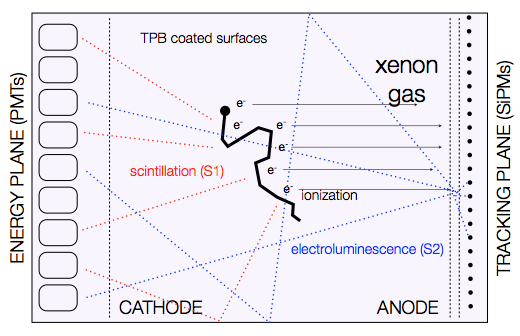
\includegraphics[width=0.9\textwidth]{img2/EL.png}
\caption{\small Principle of operation of an HPXe-EL TPC. 
} \label{fig.EL}
\end{figure}

The \emph{Neutrino Experiment with a Xenon TPC} (NEXT)\footnote{http://next.ific.uv.es/next/}  is a \bbonu\ experiment, using high-pressure (15 bar) xenon (enriched at 90\% in \XE) gas TPC with electroluminescent (EL) amplification of the ionisation signal. 

Figure \ref{fig.EL} shows the principle of operation of an HPXE-EL TPC. The detection process involves the use of the prompt scintillation light from the gas as start-of-event time, and the drift of the ionisation charge to the anode by means of an electric field ($\sim0.3$ kV/cm at 15 bar) where secondary EL scintillation is produced in the region defined by two highly transparent meshes, between which there is a field of $\sim20$ kV/cm at 15 bar. The detection of EL light provides an energy measurement using photomultipliers (PMTs) located behind the cathode (the \emph{energy plane}) as well as tracking through its detection a few mm away from production at the anode, via a dense array of silicon photomultipliers (the \emph{tracking plane}).

\subsection{NEXT prototypes}

\begin{figure}
\centering
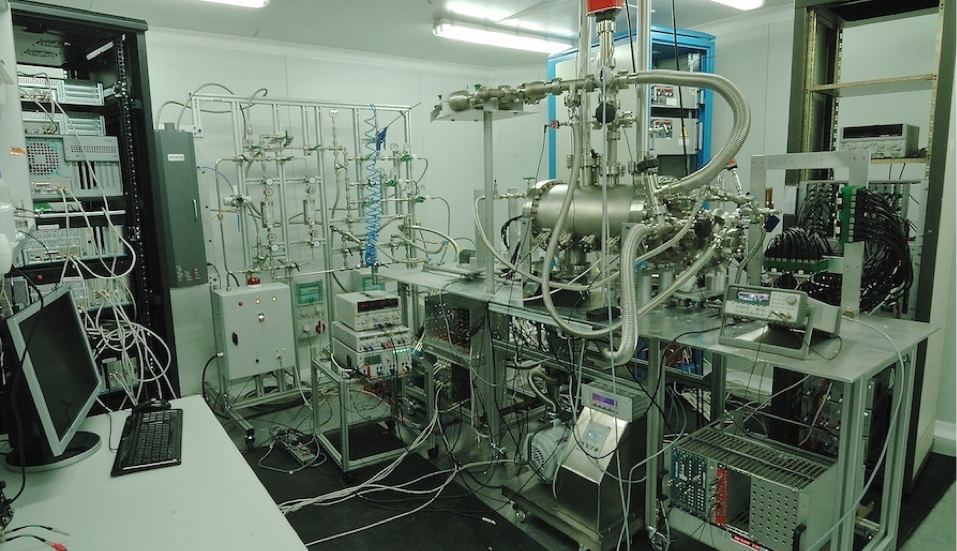
\includegraphics[width=0.9\textwidth]{img2/DemoSetup.png}
\caption{\small The NEXT-DEMO setup at IFIC (Valencia, Spain).} \label{fig.DEMO}
\end{figure}
%%%%%%%%%%
%
\begin{figure}
\centering
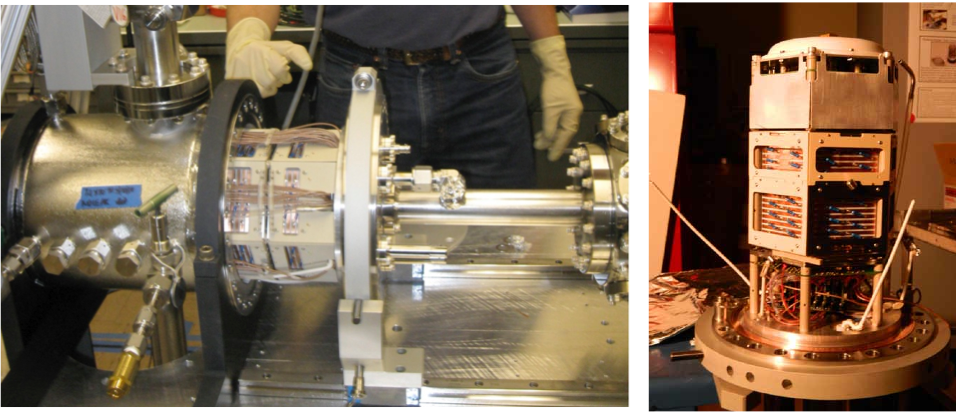
\includegraphics[width=0.9\textwidth]{img2/DBDM.png}
\caption{\small The NEXT-DBDM prototype. Top-left: the pressure vessel, in the moment in which the field cage is inserted; (b) the field cage.} \label{fig.DBDM}
\end{figure}

NEXT-DEMO, shown in figure \ref{fig.DEMO}, is as demonstrator of the HPXe-EL concept. The pressure vessel has a length of 60 cm and a diameter of 30 cm. The vessel can withstand a pressure of up to 15 bar and hosts typically 1-2 kg of xenon. NEXT-DEMO is  equipped with an energy plane made of 19 Hamamatsu R7378A PMTs and a tracking plane made of 256 Hamamatsu SiPMs. 

The detector has been operating successfully for more than four years and has demonstrated: (a) excellent operational stability, with no leaks and very few sparks; (b) good energy resolution; (c) track reconstruction with PMTs and with SiPMs coated with TPB; (d) excellent electron drift lifetime, of the order of 20 ms\cite{Alvarez:2012xda,Alvarez:2013gxa,Alvarez:2012hu}. The collaboration has just published an new article demonstrating with data the rejection power of the topological signature\cite{PFerrario:2015ina}.

The NEXT-DBDM prototype is a smaller chamber, with only 8 cm drift, but an aspect ratio (ratio diameter to length) similar to that of NEXT-100. The device has been used to perform detailed energy resolution studies, as well as studies to characterise neutrons in an \HPXE. NEXT-DBDM achieves a resolution of 1\% FWHM at 660 keV and 15 bar, which extrapolates to 0.5\% at \Qbb\cite{Alvarez:2012kua}.

\subsection{Topological signature}

%%%%%
\begin{figure}
\centering
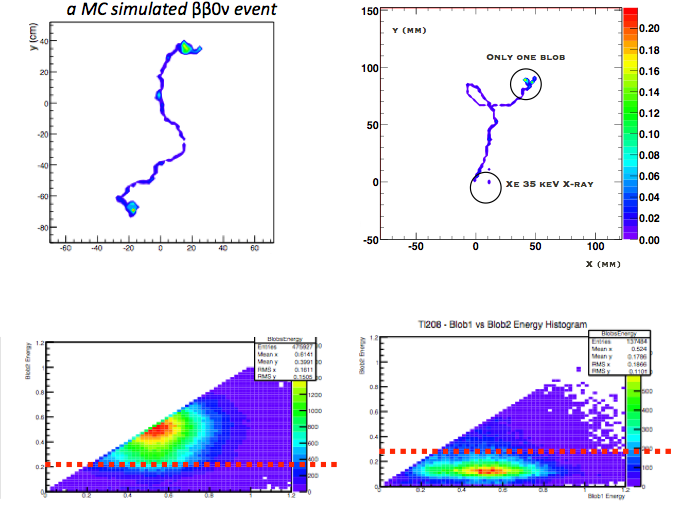
\includegraphics[width=0.9\textwidth]{img2/Topo2.png}
\caption{\small NEXT has a topological signature, not available in most \bbonu\ detectors. The top panels show the reconstruction of a Monte Carlo signal event, consisting in two electrons emanating from a common vertex (top left) and background event consisting in a single electron emitted by \BI\ or \TL\ decay (top right). The signal has two blobs of energy deposition in the track extremes, while the background has a single blob. The bottom panels show an scatter plot the energy of the blobs in the extreme of the tracks. In the case of the signal (bottom left) the energy of both blobs is high and about the same. In the case of background (top right) the energy of one blob is very small.  A simple cut requiring that the energy of both blobs is larger than a certain value (e.g, $\sim$0.2 MeV) separates effectively signal from backgrounds.}\label{fig.ETRK2}
\end{figure}
%%%%%

Double beta decay events leave a distinctive topological signature in HPXe: a continuous track with larger energy depositions (\emph{blobs}) at both ends due to the Bragg-like peaks in the 
d$E$/d$x$ of the stopping electrons (figure \ref{fig.ETRK2}, top left). In contrast, background electrons are produced by Compton or photoelectric interactions, and are characterised by a single blob and, often, by a satellite cluster corresponding to the emission of $\sim30$-keV fluorescence x-rays by xenon (figure \ref{fig.ETRK2}, top right).
Reconstruction of this topology using the tracking plane provides a powerful means of background rejection, as can be observed in the figure (see also section \ref{sec.bm}). The signal has two blobs of energy deposition in the track extremes, while the background has a single blob. The bottom panels show an scatter plot the energy of the blobs in the extreme of the tracks. In the case of the signal (bottom left) the energy of both blobs is high and about the same. In the case of background (top right) the energy of one blob is very small.  A simple cut requiring that the energy of both blobs is larger than a certain value (e.g, $\sim$0.2 MeV) separates effectively signal from backgrounds.

\subsection{Validation of the topological signature with DEMO data}

%%%%%
\begin{figure}
\centering
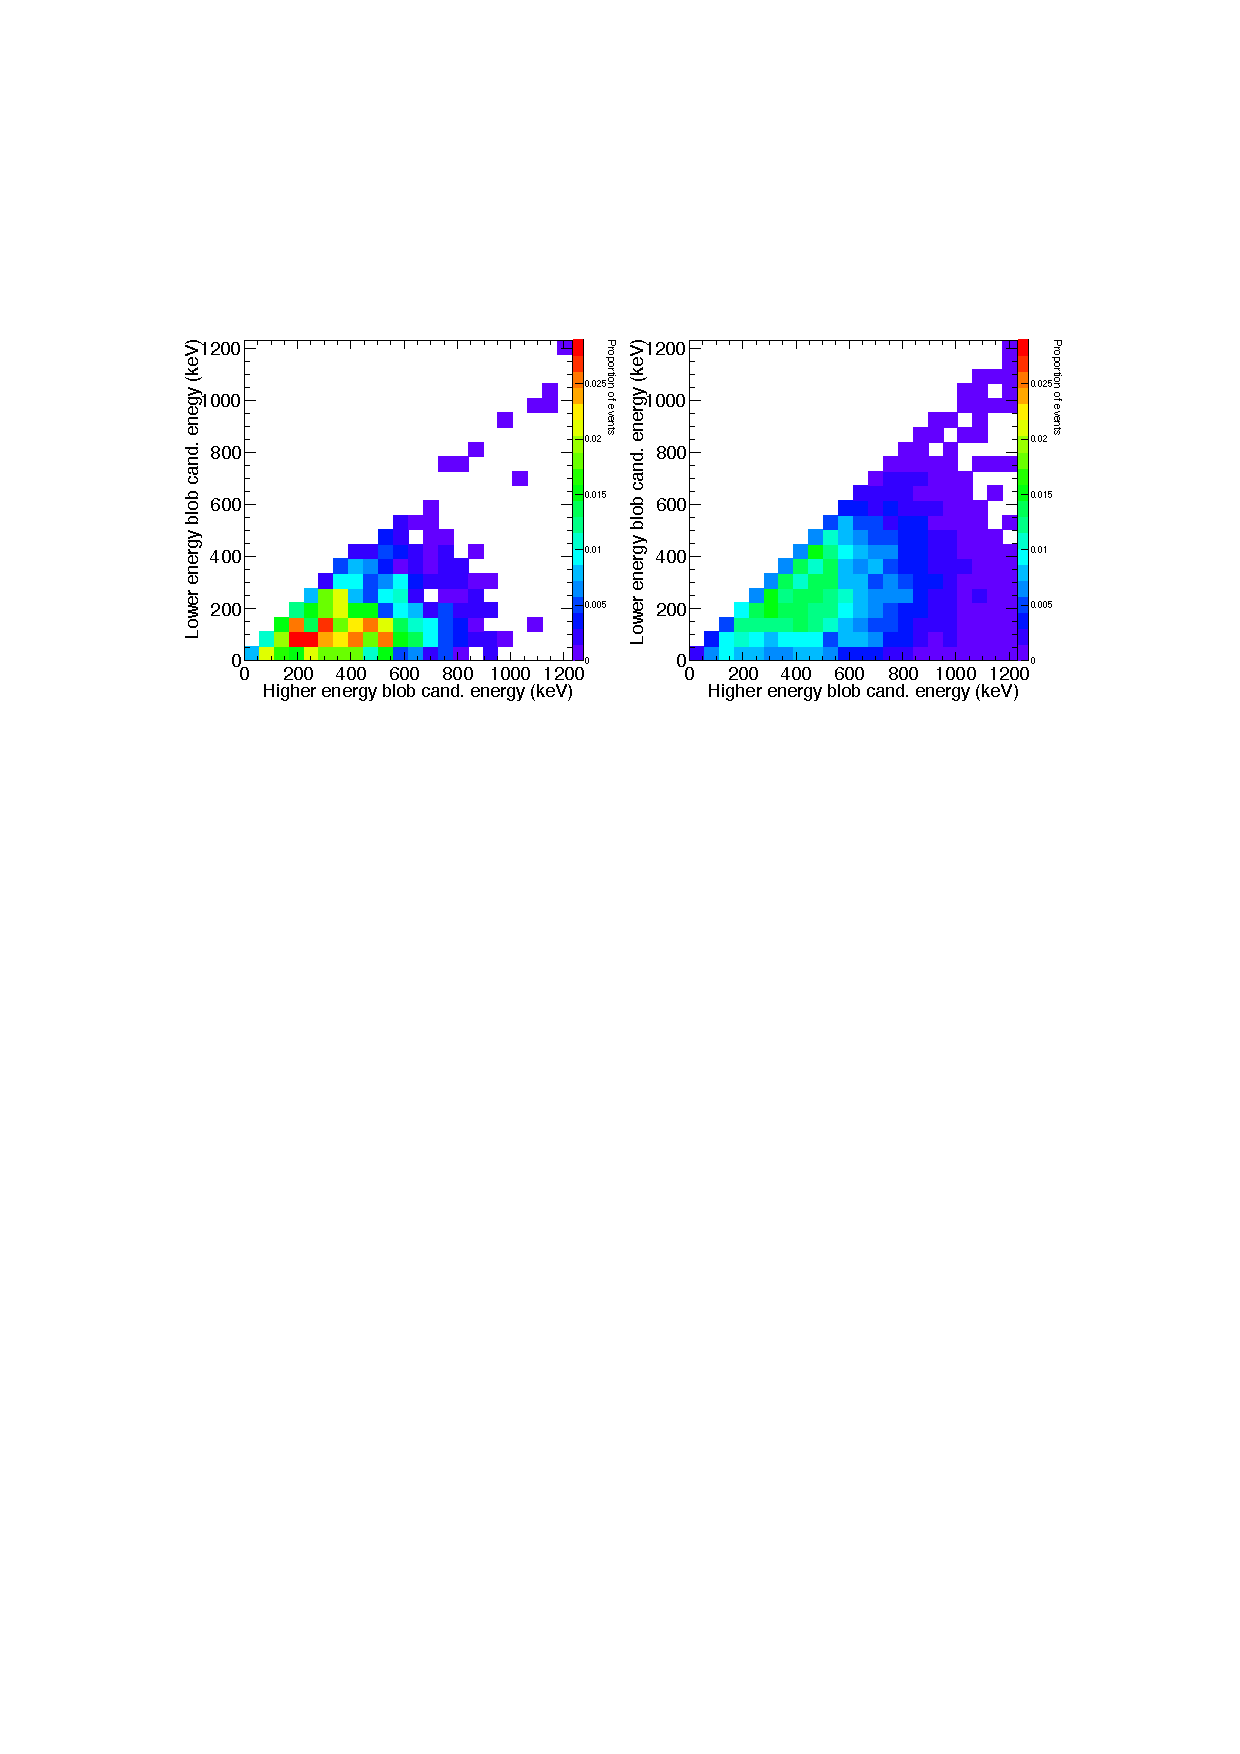
\includegraphics[width=0.9\textwidth]{img2/blobsData.pdf}
\caption{\small Energy distribution at the end-points of the tracks coming from \NA\ decay (left) and those coming from the \TL\ decay (right) for 2 cm radius blob candidates.}\label{fig.BL}
\end{figure}
%%%%% 

Figure \ref{fig.BL}, from our recently published paper \cite{PFerrario:2015ina} shows the energy distribution at the end-points of the tracks coming from \NA\ decay (left) and those coming from the \TL\ decay (right). The figure illustrates clearly that single electrons from \NA\ data are characterised by a single energetic blob, while double electrons from the double escape peak of \TL\ data show two energetic blobs. Comparison of data and Monte Carlo results using DEMO data yields an efficiency for selection \TL\ events near 70\% ($66.7 \pm 0.6$\% in data, $68.6 \pm 0.8$\% in MC). The selection efficiency for \TL\ events is smaller than for \bbonu\ events (which is around 80\%), since the tracks have less energy and thus the fraction of events with two high-energy blobs is smaller. The fraction of single electrons that pass the cut from \NA\ events is 
24\%. 

Compared to the DEMO analysis, the Monte Carlo simulation and analysis of Monte Carlo data in NEXT-100
predicts significantly improved background rejection rate of 10\% (instead of 24\%), at the same signal efficiency. A major difference which affects
these results is the relative size of the two detectors. NEXT-100 has a drift length of 1.3 m
with a circular cross section of ∼1 m and will operate at 15 bar pressure making it easily
large enough to contain electron tracks at energies similar to \Qbb\ regardless of topology
or orientation. NEXT-DEMO, on the other hand, is much smaller (the TPC has 16 cm diameter by 30 cm length). The fiducial cuts needed to contain the events tend to select tortuous tracks which do not displace as far from their origin
and are more difficult to reconstruct and more prone to blob candidate overlap. This bias,
is expected to account for the differences observed. This analysis will be repeated in 2016 with the NEW detector (see section \ref{sec.NEW}), which is only a factor two smaller than NEXT-100 (the TPC has about 0.5 m diameter and 0.5 length) and should not be affected by containment-related problems. 

\subsection{Energy resolution}

%%%%%
\begin{figure}
\centering
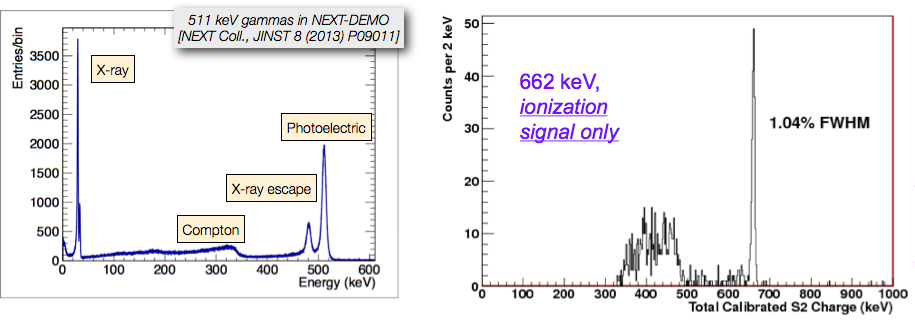
\includegraphics[width=0.9\textwidth]{img2/EResolution.png}
\caption{\small Left: the full energy spectrum measured for electrons of 511 keV in the DEMO detector. Right the spectrum near the photoelectric peak for 662 keV electrons in NEXT-DBDM. The resolution at 662 keV is 1\% FWHM (0.5\% FWHM at \Qbb). The resolution extrapolated from 511 keV is 0.7\%.}\label{fig.ERES}. 
\end{figure}
%%%%

Figure \ref{fig.ERES} shows the resolution obtained with the NEXT-DBDM apparatus. A resolution of 1\% FWHM with 
662 keV photons, has been measured, which extrapolates to 0.5\% FWHM at \Qbb. This result is not far from the expected limit obtained adding in quadrature the different factors that contribute to the resolution (Fano factor, photoelectron statistics and electronic noise). The resolution measured in NEXT-DEMO extrapolates to 0.7\% FWHM. The difference between both prototypes is due to better photoelectron statistics and aspect ratio in DBDM. The results, are, in any case, better than the target of 1\% FWHM described in the TDR. Operation with NEW (which has the same aspect ratio, roughly 1:1 than DBDM and NEXT-100) should confirm the energy resolution expected in NEXT-100. 

\subsection{NEXT-100}

\begin{figure}
\centering
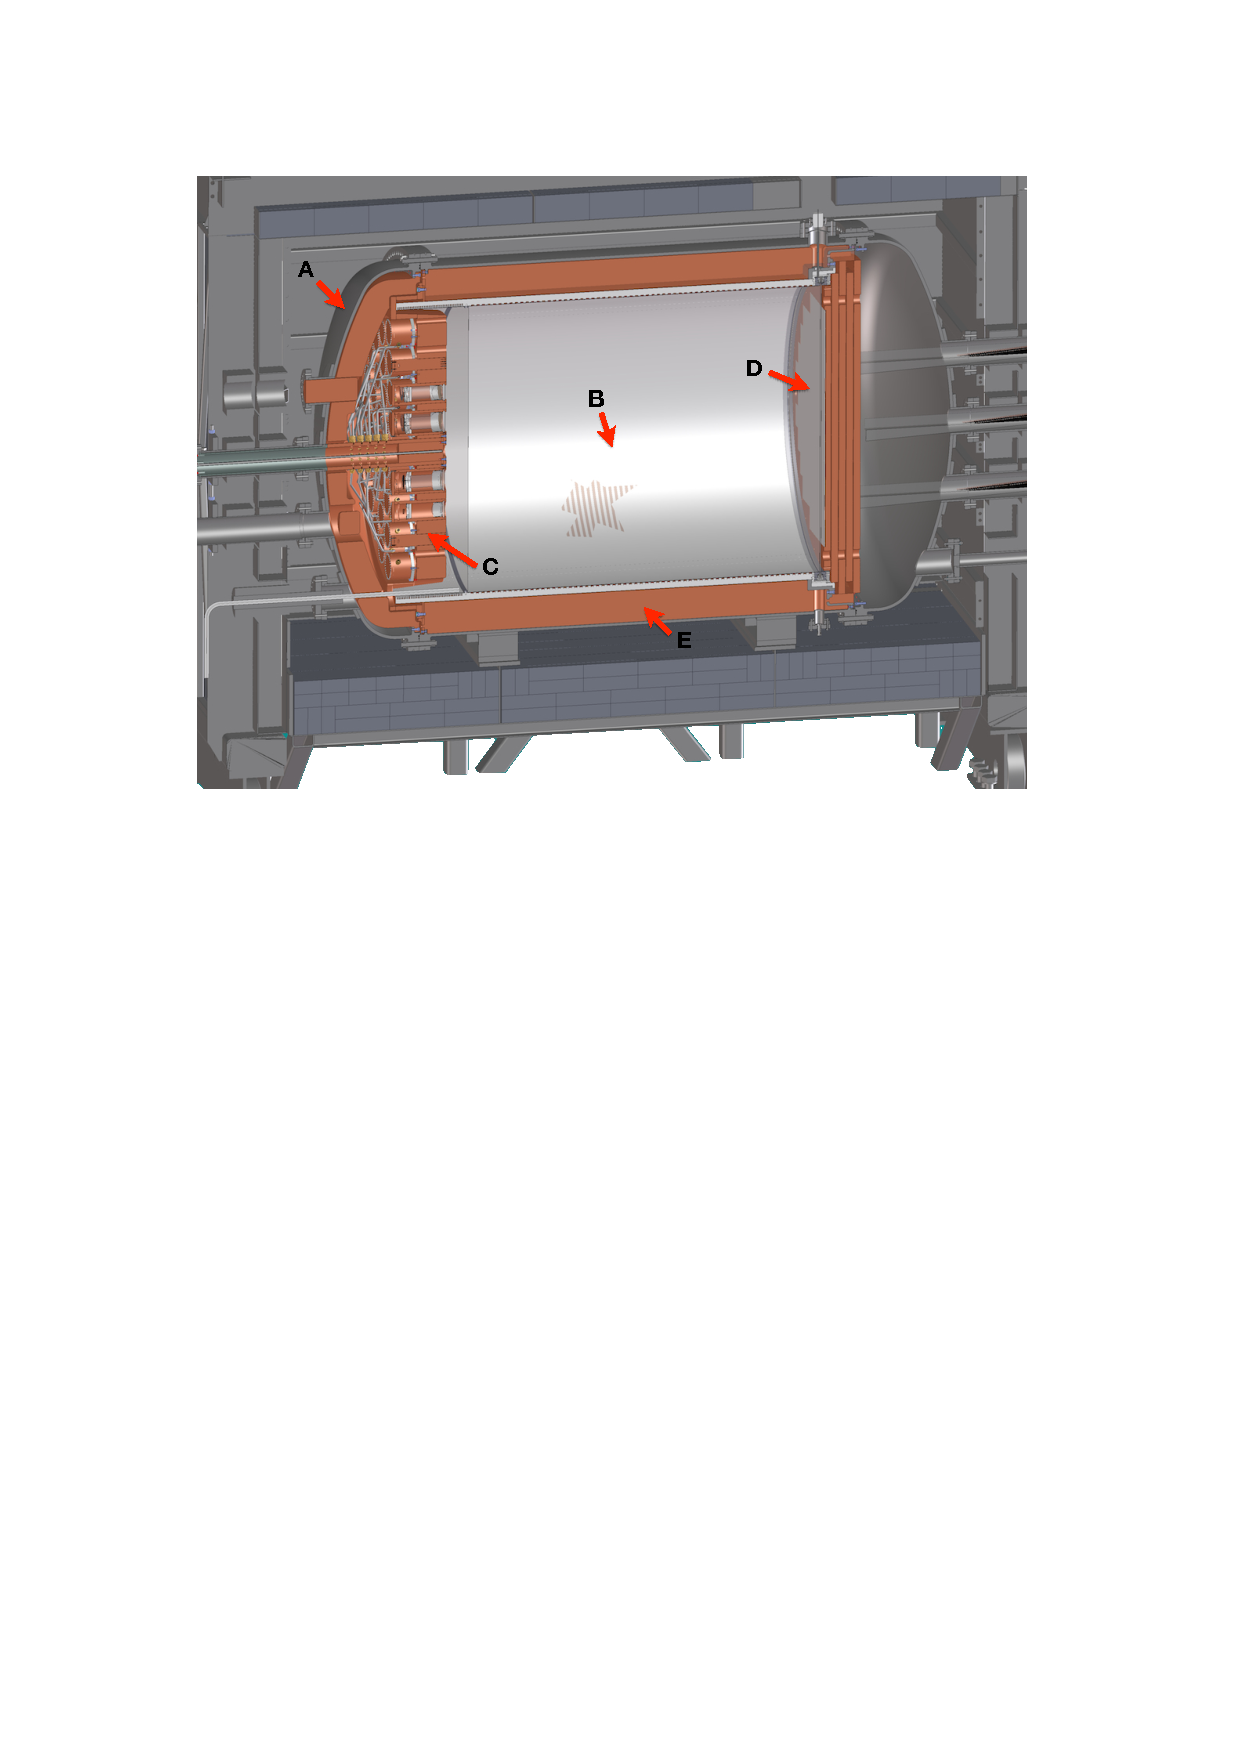
\includegraphics[width=0.9\textwidth]{img2/NEXT100.pdf}
\caption{\small Cross-section view of the NEXT-100 detector inside its lead castle shield. A stainless-steel pressure vessel (A) houses the electric-field cage (B) and the two sensor planes (energy plane, C; tracking plane, D) located at opposite ends of the chamber. The active volume is shielded from external radiation by at least 12 cm of copper (E) in all directions.
} \label{fig.NEXT100}
\end{figure}

Figure \ref{fig.NEXT100} shows a longitudinal cross-section drawing of NEXT-100 with its main components labelled. The active volume of the detector is a cylinder of approximately 1.15 m$^3$ than can hold about 100 kg of xenon gas at 15 bar. It is surrounded by an open-ended high-density polyethylene (HDPE) cylindric shell, 2.5 cm thick, 148 cm long and 107.5 cm in diameter, that provides structural stiffness and electric insulation. A series of copper rings for electric field shaping are fixed to the inner surface of the cylinder. The rings are covered by polytetrafluoroethylene (PTFE) tiles coated with tetraphenyl-butadiene (TPB) to shift the xenon VUV light to blue so as to improve the light collection efficiency. One of the ends of the HDPE cylinder is closed by a fused-silica window 1 cm thick. This window functions as the TPC anode thanks to a transparent, conductive, wavelength-shifting coating of indium tin oxide (ITO) and TPB. The two other electrodes of the TPC, EL gate and cathode, are positioned 0.5 cm and 106.5 cm away from the anode, respectively. They are built with highly transparent stainless steel wire mesh stretched over circular frames. The electrodes will be set at voltages such that a moderate electric field of 0.3--0.5 kV cm$^{−1}$~ is established in the drift region between cathode and gate, and another field of higher intensity, 2--3 kV cm$^{−1}$~ bar$^{−1}$, is created in the EL gap, between gate and anode, for the amplification of the ionization signal. The high voltage is supplied to the electrodes via radiopure, custom-made feed-throughs.

The energy plane of NEXT-100 is composed of 60 Hamamatsu R11410-10 photo-multiplier tubes located behind the cathode of the TPC and covering approximately 30\% of its area. This coverage is a compromise between the need to collect as much light as possible for a robust measurement of the energy and t$_0$, and the need to minimize the number of sensors to reduce cost, technical complexity and radioactivity. The R11410-10 is a 3-inch PMT specially developed for low-background operation. It is equipped with a synthetic silica window and a photocathode made of low temperature bialkali with quantum efficiency above 30\% for the emission wavelengths of xenon and TPB. Pressure-resistance tests run by the manufacturer showed that the R11410-10 cannot withstand pressures above 6 atmospheres. Therefore, in NEXT-100 they will be sealed into individual pressure--resistant, vacuum--tight copper enclosures closed with sapphire windows 5 mm thick. The PMTs are optically coupled to the windows using an optical gel with a refractive index intermediate between those of fused silica and sapphire. The external face of the enclosure windows is coated with TPB. The enclosures are all connected via vacuum-tight tubing conduits to a central manifold and maintained at vacuum. The PMT cables route through the conduits and the central manifold to a feedthrough in the pressure vessel nozzle.

\begin{figure}
\centering
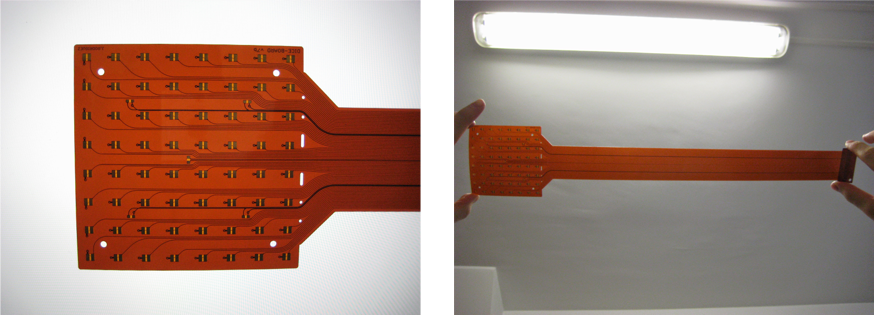
\includegraphics[width=0.9\textwidth]{img2/KDB.png}
\caption{\small The NEXT Kapton Dice Boards (KDB).} \label{fig.KDB}
\end{figure} 

The tracking function in NEXT-100 will be provided by a matrix of silicon photomultipliers (SiPMs) regularly positioned at a pitch of 1 cm and located behind the fused-silica window that closes the EL gap. The SiPMs, manufactured by SensL, have an active area of 1 mm$^2$, sensitive cells of 50 $\mu$m size, and high photon detection efficiency in the blue region (about 40\% at 440 nm). SiPMs are very cost-effective and their radioactivity is very low, given their composition (mostly silicon) and small mass. The SiPMs will be mounted on 8 × 8 flexible circuit boards made of Kapton and copper (Figure \ref{fig.KDB}). The boards have long tails that carry the signals through zigzagging slits ---so as to avoid a straight path for external gammas--- made in the copper plates that shield the active volume. The tails are connected to flat shielded cables that extract the signals from the vessel via large custom-made feed-throughs. In total, the NEXT-100 tracking plane will be composed of 7168 SiPMs distributed between 112 boards.

The sensor planes and the electric-field cage are contained within a stainless-steel pressure vessel that consists of a cylindrical central shell of 160 cm length, 136 cm inner diameter and 1 cm wall thickness, and two identical torispherical heads of 35 cm height, 136 cm inner diameter and 1 cm wall thickness. It has been fabricated with stainless steel Type 316Ti due to its low levels of natural radioactive contaminants. Designed almost entirely by the Collaboration following the ASME Pressure Vessel Code, the vessel has been built by a specialized company based in Madrid. The field cage is surrounded by a set of 12-cm thick copper bars parallel to the TPC symmetry axis, and both sensor planes are mounted to copper plates of 12 cm thickness attached to internal flanges of the vessel heads. The active volume of the detector is, therefore, shielded from external radiation by at least 12 cm of copper in all directions. The vessel sits on top of an anti-seismic pedetal and inside of a 20-cm thick lead shield made of staggered lead bricks held by a stainless-steel frame.


\section{NEXT background model and expected sensitivity to \mbb} 
\label{sec.bm}

%%%%%%%%%%%%%%%%%%%%%%%%%%%%%%%%%%%%%%%%%%%%%%%%%%%%%%%%%%%%


\subsection{Sources of backgrounds in NEXT} \label{sec:SignalAndBackground}
%%%

%%%%%%%%%%%
%\begin{figure}
%\centering
%\includegraphics[width=\textwidth]{img/TrackSignature.pdf}
%\caption{Monte Carlo simulation of signal (\bbonu\ decay of \Xe) and background (single electron of energy equal to the $Q$ value of \Xe) events in gaseous xenon at 15~bar. The ionization tracks left by signal events feature large energy deposits (or \emph{blobs}) at both ends.} \label{fig:TrackSignature}
%\end{figure}
%%%%%%%%%%

The relevance of any potential background source in NEXT depends on its probability to generate a signal-like track in the active volume of the detector with energy around the $Q$ value of \Xe. In principle, charged particles (muons, betas, etc.) entering the detector can be eliminated with essentially perfect efficiency defining a small veto region (of a few centimetres) around the boundaries of the active volume. Confined tracks generated by external neutral particles (such as high-energy gamma rays) or by internal contamination in the xenon gas can be suppressed taking advantage of both the excellent energy resolution of the detector and the topological signature.  


%%%%%%%%%%%%%%%%%%%%%%%%%%%%%%
\subsubsection*{High-energy gamma rays}
%%%
Natural radioactivity in detector materials and surroundings is, as in most other \bbonu-decay experiments, the main source of background in NEXT. In particular, the hypothetical \bbonu\ peak of \Xe\ ($\Qbb=2458.1\pm0.3$~keV lies in between the photo-peaks of the high-energy gammas emitted after the $\beta$ decays of \Bi\ and \Tl, intermediate products of the uranium and thorium series, respectively. 

The daughter isotope of \Bi, $^{214}$Po, emits a number of de-excitation gammas with energies around and above the $Q$ value of \Xe. Most of these gamma lines have very low intensity, and hence their contribution to the background rate is negligible. The gamma of 2447~keV (1.57\% intensity), however, is very close to \Qbb. Its photoelectric peak overlaps the signal peak even for energy resolutions as good as 0.5\% FWHM. The decay product of \Tl, $^{208}$Pb, emits a de-excitation photon of 2615~keV with an intensity of 99.75\%. Electron tracks from its photo-peak can lose energy via bremsstrahlung and fall in the \emph{region of interest} (ROI) around \Qbb\ defined by the energy resolution of the detector. Additionally, even though the Compton edge of the 2.6-MeV gamma is at 2382~keV, well below \Qbb, the Compton-scattered photon can generate other electron tracks close enough to the initial Compton electron to be reconstructed as a single track with energy around \Qbb. 

%%% TABLE %%%%%%%%%%%%%%%%%%%%
%%%%%%%%%%%%%%%%%%%%%%%%%%%%%%%%%%%%%%%%%%%%%%%%%%%%%%%%%%%%

%%%%%%%%%%
\begin{table}
\centering
{\small
\begin{tabular}{l l l l D{.}{.}{2.9} D{.}{.}{2.9}}
\toprule
%
Material & Subsystem & Technique & Units & \multicolumn{1}{l}{\Tl} & \multicolumn{1}{l}{\Bi} \\ \midrule
%
Copper (CuA1) & IS, EP, FC & GDMS & mBq/kg & <0.0014 & <0.012 \\
%
Fused silica & FC & NAA & mBq/kg & 0.0097(18) & 0.07(3) \\
%
Kapton board & TP & HPGe & mBq/unit & 0.0104(11) & 0.070(5) \\
%
Lead & OS & GDMS & mBq/kg & 0.034(7) & 0.35(7) \\
%
PMT R11410-10 & EP & HPGe & mBq/PMT & 0.30(9) & <0.94 \\
%
Polyethelene & FC & ICPMS & mBq/kg & <0.0076 & <0.062 \\
%
Resistor (1~G$\Omega$) & FC & HPGe & mBq/unit & 0.000011(6) & 0.00009(4) \\
%
Sapphire & EP & NAA & mBq/unit & 0.04(1) & <0.31 \\
%
Steel (316Ti) & PV & GDMS, HPGe & mBq/kg & <0.15 & <0.46 \\
%
SiPM SensL & TP & HPGe & mBq/unit & <0.00003 & <0.00009 \\
\bottomrule
\end{tabular} }
\caption{Specific activity of \Tl\ and \Bi\ in the most relevant materials and components used in the NEXT-100 detector \cite{Alvarez:2012as, Alvarez:2014kvs}. Three items (fused silica, sapphire and the field-cage resistors) have not been screened yet with sufficient precision; therefore, we use instead  measurements by the EXO Collaboration \cite{Leonard:2007uv, Auger:2012gs}. The activities determined via mass spectrometry (GDMS or ICPMS) or neutron activation analysis (NAA) were derived from Th and U concentrations. High-purity germanium (HPGe) $\gamma$-ray spectroscopy results correspond, whenever possible, to the lower parts of the natural decay chains. The figures in parentheses after the measurements give the 1-standard-deviation uncertainties in the last digits; the limits are given at 95\% CL. The abbreviations used to refer to the NEXT-100 detector subsystems have the following meaning: EP: energy plane; TP: tracking plane; FC: electric-field cage; PV: pressure vessel; IS: inner shielding; OS: outer shielding.} \label{tab:SpecificActivity}
\end{table}
%%%%%%%%%%

%%%%%%%%%%%%%%%%%%%%%%%%%%%%%%%%%%%%%%%%%%%%%%%%%%%%%%%%%%%% % \label{tab:SpecificActivity}
%%%%%%%%%%%%%%%%%%%%%%%%%%%%%%

%%% TABLE %%%%%%%%%%%%%%%%%%%%

%%%%%%%%%%
\begin{table}[!]
\centering
\begin{tabular}{lll c c}
\toprule
Detector subsystem & Material & Quantity & \multicolumn{1}{c}{\Tl} & \Bi\ \\ 
                   &          &          & \multicolumn{1}{c}{(mBq)} & (mBq) \\ \midrule
%
\emph{Pressure vessel} \\
\quad Total & Steel 316Ti & 1310~kg & $<197$ & $<603$ \\ \addlinespace
%
\emph{Energy plane} \\
%
\quad PMTs & R11410-10 & 60~units & $12(3)$ & $<56$ \\
\quad PMT enclosures & Copper CuA1 & 60$\times$4.3 kg & $<0.36$ & $<3.1$ \\
\quad Enclosure windows & Sapphire & 60$\times$0.14 kg & $0.34(8)$ & $<2.6$ \\ 
\quad Support plate & Copper CuA1 & 408~kg & $<0.6$ & $<5$ \\ \addlinespace 
%
\emph{Tracking plane} \\
%
\quad SiPMs & {\scshape Sensl} 1~mm$^{2}$ & 107$\times$64 units & $<5$ & $<18$ \\
\quad Boards & Kapton FPC & 107 units & $1.5(2)$ & $3.2(1.1)$ \\ \addlinespace 
%
\emph{Field cage} \\
%
\quad Barrel & Polyethylene & 128~kg & $<1$ & $<8$ \\
\quad Shaping rings & Copper CuA1 & 120$\times$3~kg & $<0.5$ & $<4$ \\
\quad Electrode rings & Steel 316Ti & 2$\times$5~kg & $1.5$ & $<5$ \\
\quad Anode plate & Fused silica & 9.5~kg & $0.092(17)$ & $0.7(3)$ \\
\quad Resistor chain & 1-G$\Omega$ resistors & 240 units & $<0.0026$ & $<0.020$ \\ \addlinespace
%
\emph{Shielding} \\
%
\quad Inner shield & Copper CuA1 & 9210~kg & $<13$ & $<111$ \\
\quad Outer shield & Lead & 60700~kg & $2060(430)$ & 21300(4300) \\
\bottomrule
\end{tabular}
\caption{Radioactivity budget of the NEXT-100 detector. The figures in parentheses after the measurements give the 1-sigma uncertainties in the last digit. The upper limits in the activity of most subsystems originate in the 95\% CL limits set on the specific activity of the corresponding materials quoted on Table~\ref{tab:SpecificActivity}.} \label{tab:RadioactiveBudget}
\end{table}
%%%%%%%%%% % \label{tab:RadioactiveBudget}
%%%%%%%%%%%%%%%%%%%%%%%%%%%%%%

The NEXT Collaboration is carrying out a thorough campaign of material screening and selection using gamma-ray spectroscopy (with the assistance of the LSC Radiopurity Service) and mass spectrometry techniques (ICPMS and GDMS). Table~\ref{tab:SpecificActivity} collects the measurements of the specific activity of \Tl\ and \Bi\ in the most relevant materials and components used in the NEXT-100 detector, and Table~\ref{tab:RadioactiveBudget} details the radioactivity budget of NEXT-100 separated into detector subsystems.

The rock walls of the underground laboratory are a rather intense source of high-energy gammas due to the presence of trace radioactive contaminants in their composition. The total gamma flux in Hall A at LSC is $1.06\pm0.24$~cm$^{-2}$~s$^{-1}$, with contributions from $^{40}$K ($0.52\pm0.23$~cm$^{-2}$~s$^{-1}$), $^{238}$U ($0.35\pm0.03$~cm$^{-2}$~s$^{-1}$) and $^{232}$Th ($0.19\pm0.04$~cm$^{-2}$~s$^{-1}$). Nevertheless, the external lead shield of NEXT-100 will attenuate this flux by more than 4 orders of magnitude, making its contribution to the final background rate negligible. 

%%%%%%%%%%%%%%%%%%%%%%%%%%%%%%
\subsubsection*{Radon}
%%%

The measured activity of airborne radon ($^{222}$Rn) at the Laboratorio Subterr\'aneo de Canfranc (Hall A) varies between 60 and 80~mBq~m$^{-3}$. Left at this level, radon would represent an intolerably high source of gamma rays from \Bi. For this reason, the vicinity of the detector (the internal volume of the lead castle shield) will be flushed with clean air produced by a radon mitigation system such as those used, for instance, by the NEMO-3 and DarkSide experiments. A reduction of, at least, a factor of 100 in the activity of airborne radon is expected.

Radon can also emanate from detector components and be transported to the active volume through the gas circulation. The $\alpha$ decays of radon (either $^{220}$Rn or $^{222}$Rn) in the bulk xenon do not represent a background: they have energies well above \Qbb\ and their very short tracks are easily identified \cite{Alvarez:2012hu}. The progeny of radon is positively charged and will drift toward the TPC cathode. A majority of the subsequent \Bi\ and \Tl\ beta decays will occur on the cathode rather than in the active volume. These cathode events are equivalent to other background sources close to the active volume (\Tl\ and \Bi\ decays from the sensor planes, for instance): if the $\beta$ particle enters the active volume, the event can then be vetoed; otherwise, the de-excitation gamma rays that interact in the xenon can generate background tracks. In addition, a small fraction (0.2\%) of the \Bi\ $\beta$ decays occurring in the xenon bulk will produce an electron track with energy around \Qbb. Luckily, the disintegration of \Bi\ is followed shortly after by the $\alpha$ decay of $^{214}$Po ($T_{1/2} = 164~\mu$s \cite{Wu:2012nds}). The detection of this so-called Bi-Po coincidence can be used to identify and suppress with high efficiency these background events.

The design of NEXT-100 minimizes the use of materials and components known to emanate radon in high rates, such as plastics, cables or certain seals. Nevertheless, estimating a priori the emanation rate and radon activity in the xenon is difficult, since the available data are scant and have been acquired in very different conditions (in vacuum, typically). Understanding the impact of radon emanation and its suppression---by means of a radon trap, for example---is one of the priorities of the NEW program (see section \ref{sec.new}).

%%%%%%%%%%%%%%%%%%%%%%%%%%%%%%%%%%%%%%%%%%%%%%%%%%%%%%%%%%%%
\subsection{Event selection} \label{sec:EventSelection}
%%%

The criteria to accept a reconstructed event as a \bbonu-decay candidate in NEXT are the following:
%%%
\begin{enumerate}
\item The event consists of one single reconstructed track confined within the \emph{fiducial} volume of the detector ---\thinspace defined by excluding a region of 2~cm around the boundaries of the active volume\thinspace--- and with energy between 2.4 and 2.5~MeV.
\item The reconstructed track features a \emph{blob} in both ends.
\item The energy of the event is within the \emph{region of interest} (ROI) around \Qbb.
\end{enumerate}
%%%

The definition of a \emph{fiducial} volume has two purposes: it rejects all charged backgrounds entering the detector, and it discards those events in which the tracked particles may have left the active volume, depositing part of their energy in passive materials. The size of the excluded region, 2 centimetres around the boundaries of the active volume, takes into account the voxel size (which, in turn, depends on the spatial resolution of the detector) and the higher inhomogeneity of the electric field near the edges of the field cage (which may affect the quality of the reconstruction in that region). In practical terms, this fiducial cut is implemented demanding that none of the voxels located in the vetoed region contains energy above the detection threshold of the tracking plane (set, conservatively, to 10~keV).


The requirement for the accepted events to have one and only one reconstructed track takes advantage of the very different track multiplicities ---\thinspace that is, the number of reconstructed tracks per event\thinspace--- of signal and background. Approximately 70\% of the signal events satisfy the single-track condition, whereas only 10\% of \Tl\ and \Bi\ events do so. 

Next, we exploit the characteristic energy-deposition pattern of \bbonu-decay tracks which feature a blob at both ends (see Figure \ref{fig.ETRK2}). We define the energy of a blob as the total energy contained in all the voxels whose center is at a maximum distance of $2$~cm with respect to the one reconstructed as track end. A simple selection requires that the energy for both blob candidates is above  0.2~MeV.

Finally, events are accepted if their energy fall inside a ROI around \Qbb, defined as the region that maximizes the ratio of the signal efficiency over the square root of the background rate.
 
 %%%%%%%%%%
\begin{figure}
\centering
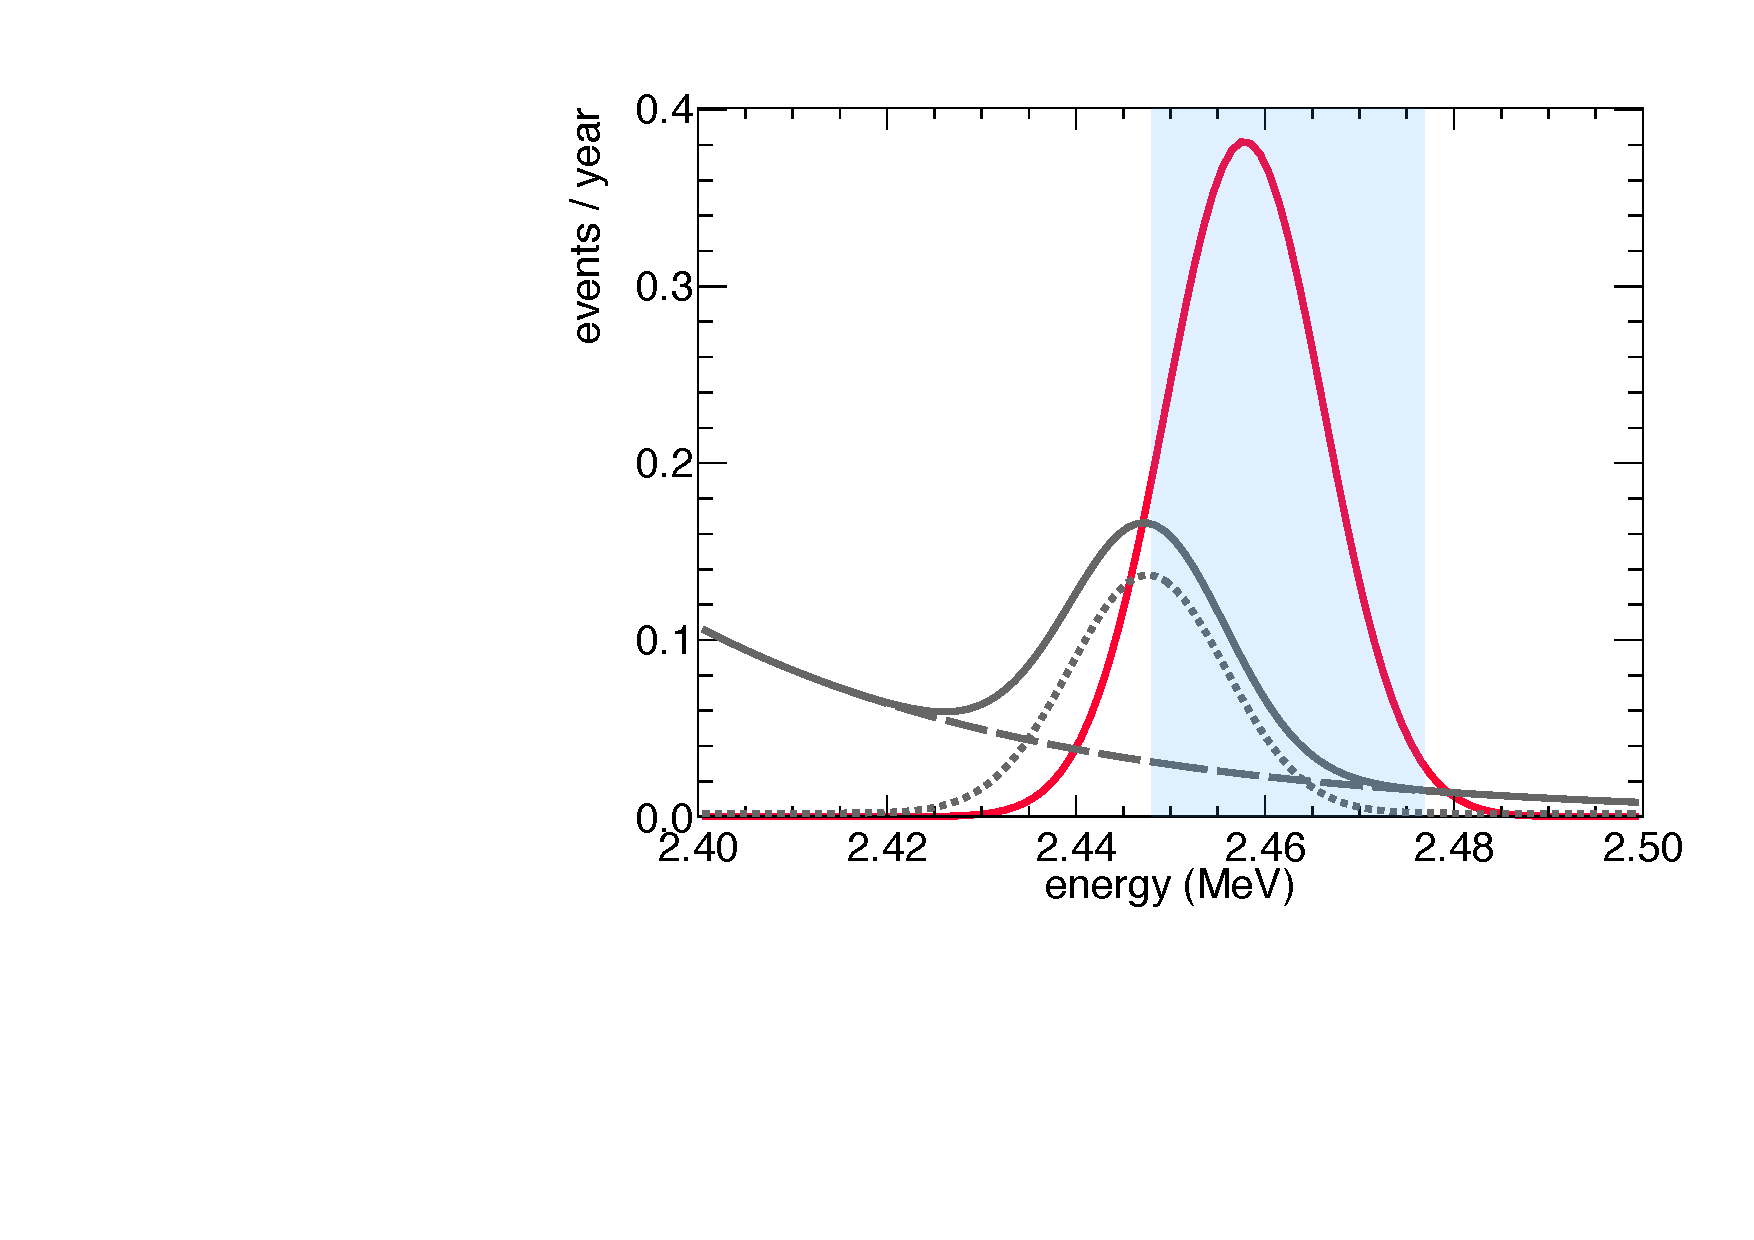
\includegraphics[width=0.9\textwidth]{img2/Next100ROI.pdf}
\caption{Energy spectra of signal (red, solid curve) and background (\Tl: grey, dashed distribution; \Bi: grey, dotted distribution; total: grey, solid distribution) in the region of interest (ROI) around \Qbb. The optimal ROI (the one that maximizes the ratio of the signal efficiency over the square root of the background rate) is indicated by the shaded, blue region. The signal strength represented here corresponds to a neutrino Majorana mass of 200 meV, while the backgrounds are scaled to their expected values in NEXT-100 ($6\times10^{-4}$~\ckky), assuming an exposure of 91~kg~yr.} \label{fig:ROI}
\end{figure}
%%%%%%%%%%


Table~\ref{tab:AcceptanceSelectionCriteria} summarizes the acceptances for signal and background of the selection criteria described above. The natural radioactive backgrounds, \TL\ and \BI, are suppressed by morel than 6 orders of magnitude, and the contribution of \bbtnu-decay to the background rate is completely negligible. The cuts yield a signal efficiency of 28\%. Note, however, that approximately half of the events are lost already in the first selection cut: 88\% of the events are contained within the fiducial volume of the detector, 71\% have one single track, and 76\% of them have reconstructed energy above 2.4~MeV (the \bbonu\ spectrum has a tail extending to low energies composed of events with missing energy in the form of bremsstrahlung radiation).

%%%%%%%%%%
\begin{table}[!]
\centering
\begin{tabular}{l c l l l}
\toprule
%
Selection criterion & \multicolumn{1}{c}{\bbonu} & \multicolumn{1}{c}{\bbtnu} & \multicolumn{1}{c}{\Tl} & \multicolumn{1}{c}{\Bi} \\ \midrule
Fiducial, single track & \multirow{2}{*}{0.4759} & \multirow{2}{*}{$8.06\times10^{-9}$} & \multirow{2}{*}{$2.83\times10^{-5}$} & \multirow{2}{*}{$1.04\times10^{-5}$} \\
$E\in[2.4, 2.5]~\mathrm{MeV}$ \\ \addlinespace
%
Track with 2 blobs & 0.6851 & 0.6851 & 0.1141 & 0.105 \\ \addlinespace
%
Energy ROI & 0.8661 & $3.89\times10^{-5}$ & 0.150 & 0.457 \\ \addlinespace
%
\emph{Total} & 0.2824 & $2.15\times10^{-13}$ & $4.9\times10^{-7}$ & $4.9\times10^{-7}$ \\
\bottomrule
\end{tabular}
\caption{Acceptance of the selection criteria for \bbonu-decay events described in the text. The values for \Tl\ and \Bi\ correspond to one of the dominant sources of background in the detector.} \label{tab:AcceptanceSelectionCriteria}
\end{table}
%%%%%%%%%%

%%%%%%%%%%%%%%%%%%%%%%%%%%%%%%%%%%%%%%%%%%%%%%%%%%%%%%%%%%%%
\subsection{Estimated background rate in NEXT-100} \label{sec:BkgRate}
%%%
The contribution of each detector subsystem to the overall background rate of NEXT-100 is shown in Table~\ref{tab:BackgroundContributions}. These rates are obtained dividing the initial activities of \Tl\ and \Bi\ by the corresponding background rejection factors (defined as the inverse of the background acceptance resulting from the \bbonu-decay event selection described in the previous section). They are also represented graphically in Figure~\ref{fig:BackgroundContributions}. The photosensors are, by far, the dominant source of background in NEXT-100. Notice, however, that our knowledge is, in any case, quite uncertain, given that for most background sources we only have at present a limit to their activity. This is, in fact, a problem common to all \bbonu-decay experiments, and it will be even more serious for the experiments of the tonne scale, which will require materials and components of higher radiopurity.


%%%%%%%%%%
\begin{sidewaystable}
\centering
\caption{Contribution to the background rate of NEXT-100 predicted for each subsystem of the detector considered in our background model. The second and third columns correspond to the initial activities of \Tl\ and \Bi\ (see Table~\ref{tab:RadioactivityBudget}). The fourth and fifth columns contain the rejection factors computed with the detector simulation. The last two columns in the table show the background rate estimated for each subsystem (i.e.\ the ratio of the previous quantities) expressed in $10^{-4}$~\ckky. For most subsystems, we only have upper limits to their induced background rate. In those cases where we have a positive measurement, the figures in parentheses give the 1-sigma uncertainty in the last digit.} \label{tab:BackgroundContributions}
%%%
\small
\begin{tabular*}{.9\textheight}{@{\extracolsep{\fill}} l *{2}{c} *{2}{l} *{2}{D{.}{.}{4.4}}}
\toprule
%%%
Detector subsystem & \multicolumn{2}{c}{Activity (mBq)} & \multicolumn{2}{c}{Rejection factor} & \multicolumn{2}{c}{$c$ $\left(\mathrm{10^{-4}/(keV~kg~yr)}\right)$} \\ \cmidrule(lr){2-3} \cmidrule(lr){4-5} \cmidrule(l){6-7}
       & \multicolumn{1}{c}{\Tl} & \multicolumn{1}{c}{\Bi} & \multicolumn{1}{c}{\Tl} & \multicolumn{1}{c}{\Bi} & \multicolumn{1}{c}{\Tl} & \multicolumn{1}{c}{\Bi} \\ \midrule
%%%
\emph{Pressure vessel} \\
%
\quad Total & $<197$ & $<603$ & $1.0(3)\times10^{8}$ & $1.0(5)\times10^{9}$ & <0.23 & <0.07 \\ \addlinespace
%%%
\emph{Energy plane} \\
%
\quad PMTs & $12(3)$ & $<56$ & $4.1(3)\times10^{6}$ & $6.1(5)\times10^{6}$ & 0.35(9) & <1.1 \\
%
\quad PMT enclosures & $<0.34$ & $<2.6$ & $6.8(6)\times10^{6}$ & $9.5(9)\times10^{6}$ & <0.006 & <0.04 \\
%
\quad Enclosure windows & $0.34(8)$ & $<2.6$ & $2.38(11)\times10^{6}$ & $2.56(13)\times10^{6}$ & 0.017(4) & <0.12 \\
%
\quad Support plate & $<0.6$ & $<5$ & $5.0(4)\times10^{6}$ & $1.43(16)\times10^{7}$ & <0.014 & <0.04 \\ \addlinespace
%%%
\emph{Tracking plane} \\
\quad SiPMs & $<5$ & $<18$ & $2.04(8)\times10^{6}$ & $2.04(8)\times10^{6}$ & <0.29 & <1.1 \\
\quad SiPM boards & $1.5(2)$ & $3.2(1.1)$ & $2.04(8)\times10^{6}$ & $2.04(8)\times10^{6}$ & 0.088(13) & 0.19(6) \\ \addlinespace
%%%
\emph{Electric-field cage} \\
\quad Barrel & $<1$ & $<8$ & $2.61(13)\times10^{6}$ & $2.27(10)\times10^{6}$ & <0.05 & <0.4 \\ 
\quad Shaping rings & $<0.5$ & $<4$ & $2.61(13)\times10^{6}$ & $2.27(10)\times10^{6}$ & <0.023 & <0.23 \\
%
\quad Electrode rings & $<1.5$ & $<5$ & $2.61(13)\times10^{6}$ & $2.27(10)\times10^{6}$ & <0.07 & < 0.24 \\
%
\quad Anode plate & $0.092(17)$ & $0.7(3)$ & $2.04(8)\times10^{6}$ & $2.04(8)\times10^{6}$ & 0.005(1) & 0.039(17) \\
%
\quad Resistor chain & $<0.0026$ & $<0.0013$ & $2.61(13)\times10^{6}$ & $2.27(10)\times10^{6}$ & <0.00012 & <0.0011 \\ \addlinespace
%%%
\emph{Shielding} \\
\quad Inner shield & $<13$ & $<111$ & $9.3(9)\times10^{6}$ & $1.9(3)\times10^{7}$ & <0.17 & <0.7 \\
\quad Outer shield & $2060(430)$ & $21300(4300)$ & $1.0(5)\times10^{10}$ & $1.0(5)\times10^{10}$ & 0.025(13) & 0.25(14) \\
\bottomrule
\end{tabular*}
\end{sidewaystable}
%%%%%%%%%%


%%%%%%%%%%
\begin{figure}
\centering
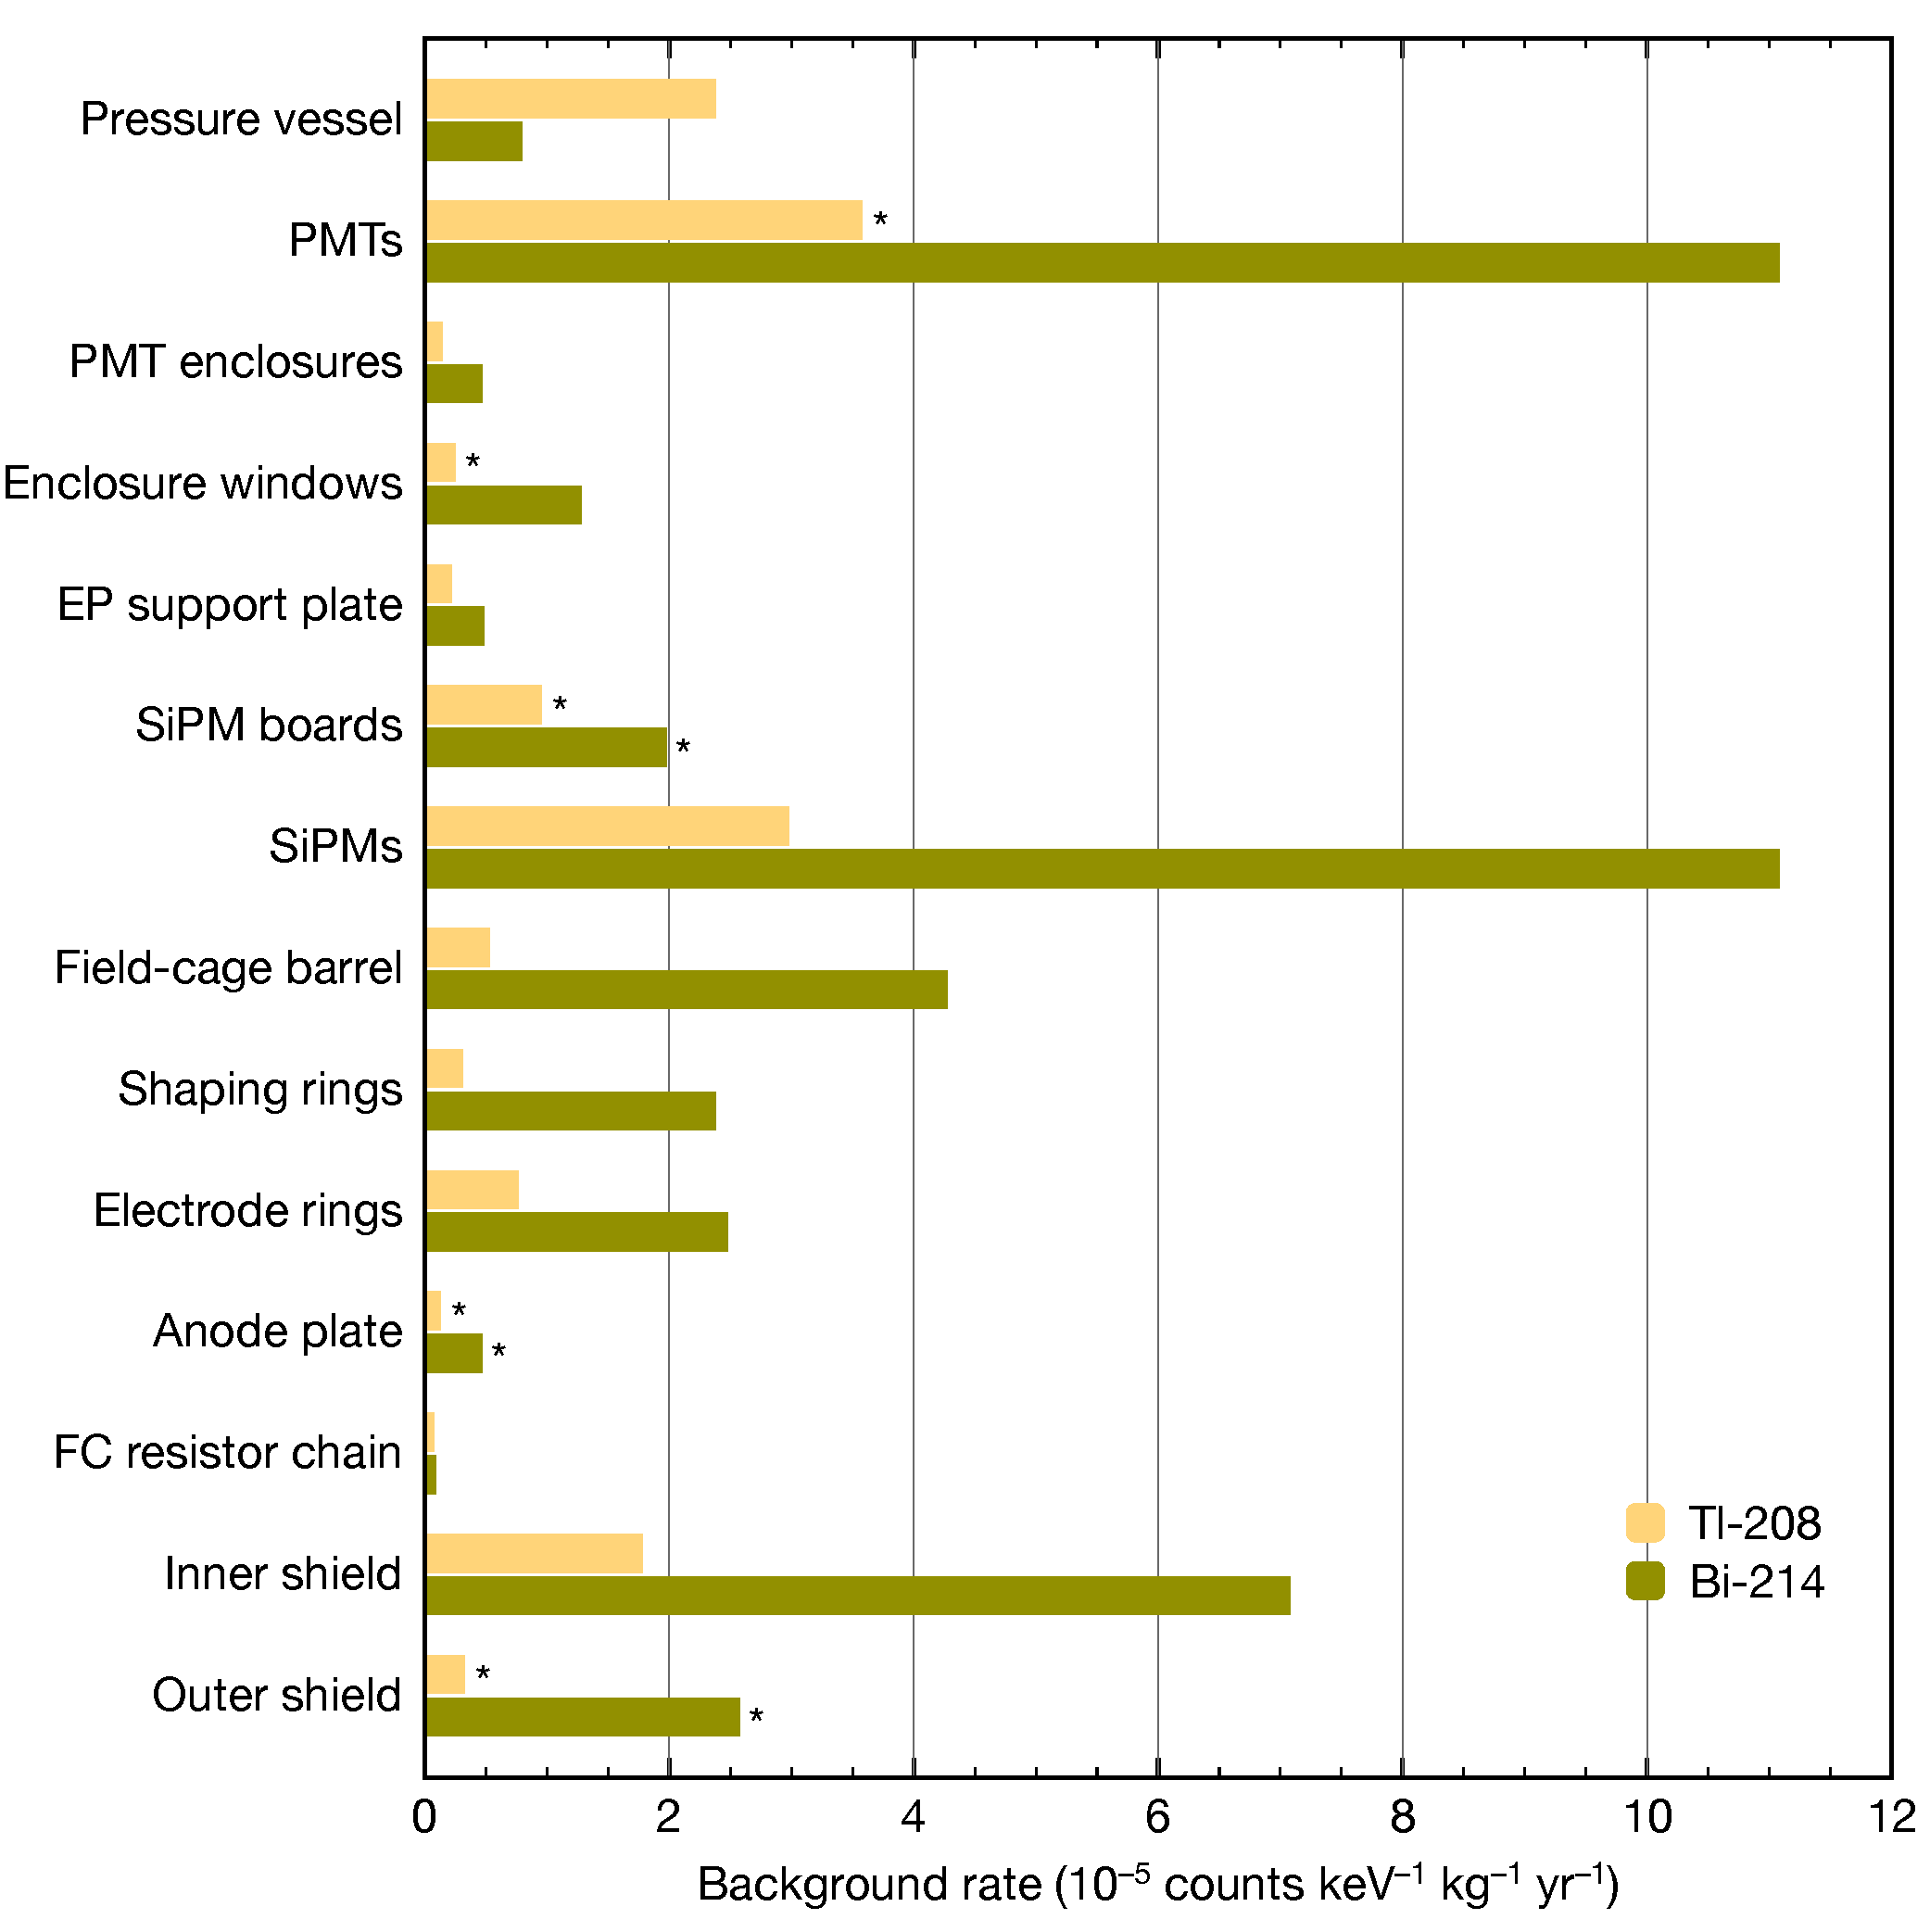
\includegraphics[width=0.9\textwidth]{img2/BackgroundSources.pdf}
\caption{Contribution to the background rate of NEXT-100 of the different detector subsystems considered in our background model. An asterisk (*) next to a bar indicates that the contribution corresponds to a positive measurement of the activity of the material.} \label{fig:BackgroundContributions}
\end{figure}
%%%%%%%%%%

%%%%%%%%%%
\begin{table}
\centering
\caption{Contribution of major subsystems to the expected background rate of NEXT-100, expressed in 10$^{-4}$ counts~keV$^{-1}$~kg$^{-1}$~yr$^{-1}$.} \label{tab:BkgRateSummary}
\begin{tabular*}{.8\textwidth}{@{\extracolsep{\fill}} l *{3}{D{.}{.}{4.6}}}
\toprule
Detector subsystem & \multicolumn{1}{c}{\Tl} & \multicolumn{1}{c}{\Bi} & \multicolumn{1}{c}{\itshape Total} \\ \midrule
Pressure vessel     & <0.23 & <0.07 & <0.31 \\
Energy plane        & <0.38 & <1.31 & <1.69 \\
Tracking plane      & <0.38 & <1.27 & <1.65 \\
Electric-field cage & <0.14 & <0.93 & <1.07 \\
Inner shield        & <0.17 & <0.70 & <0.87 \\
Outer shield        & 0.025(13) & 0.25(14) & 0.28(14) \\
{\itshape Total}    & <1.33 & <4.53 & <5.86 \\ 
\bottomrule
\end{tabular*}
\end{table}
%%%%%%%%%%

%%%%%%%%%%
\begin{figure}
\centering
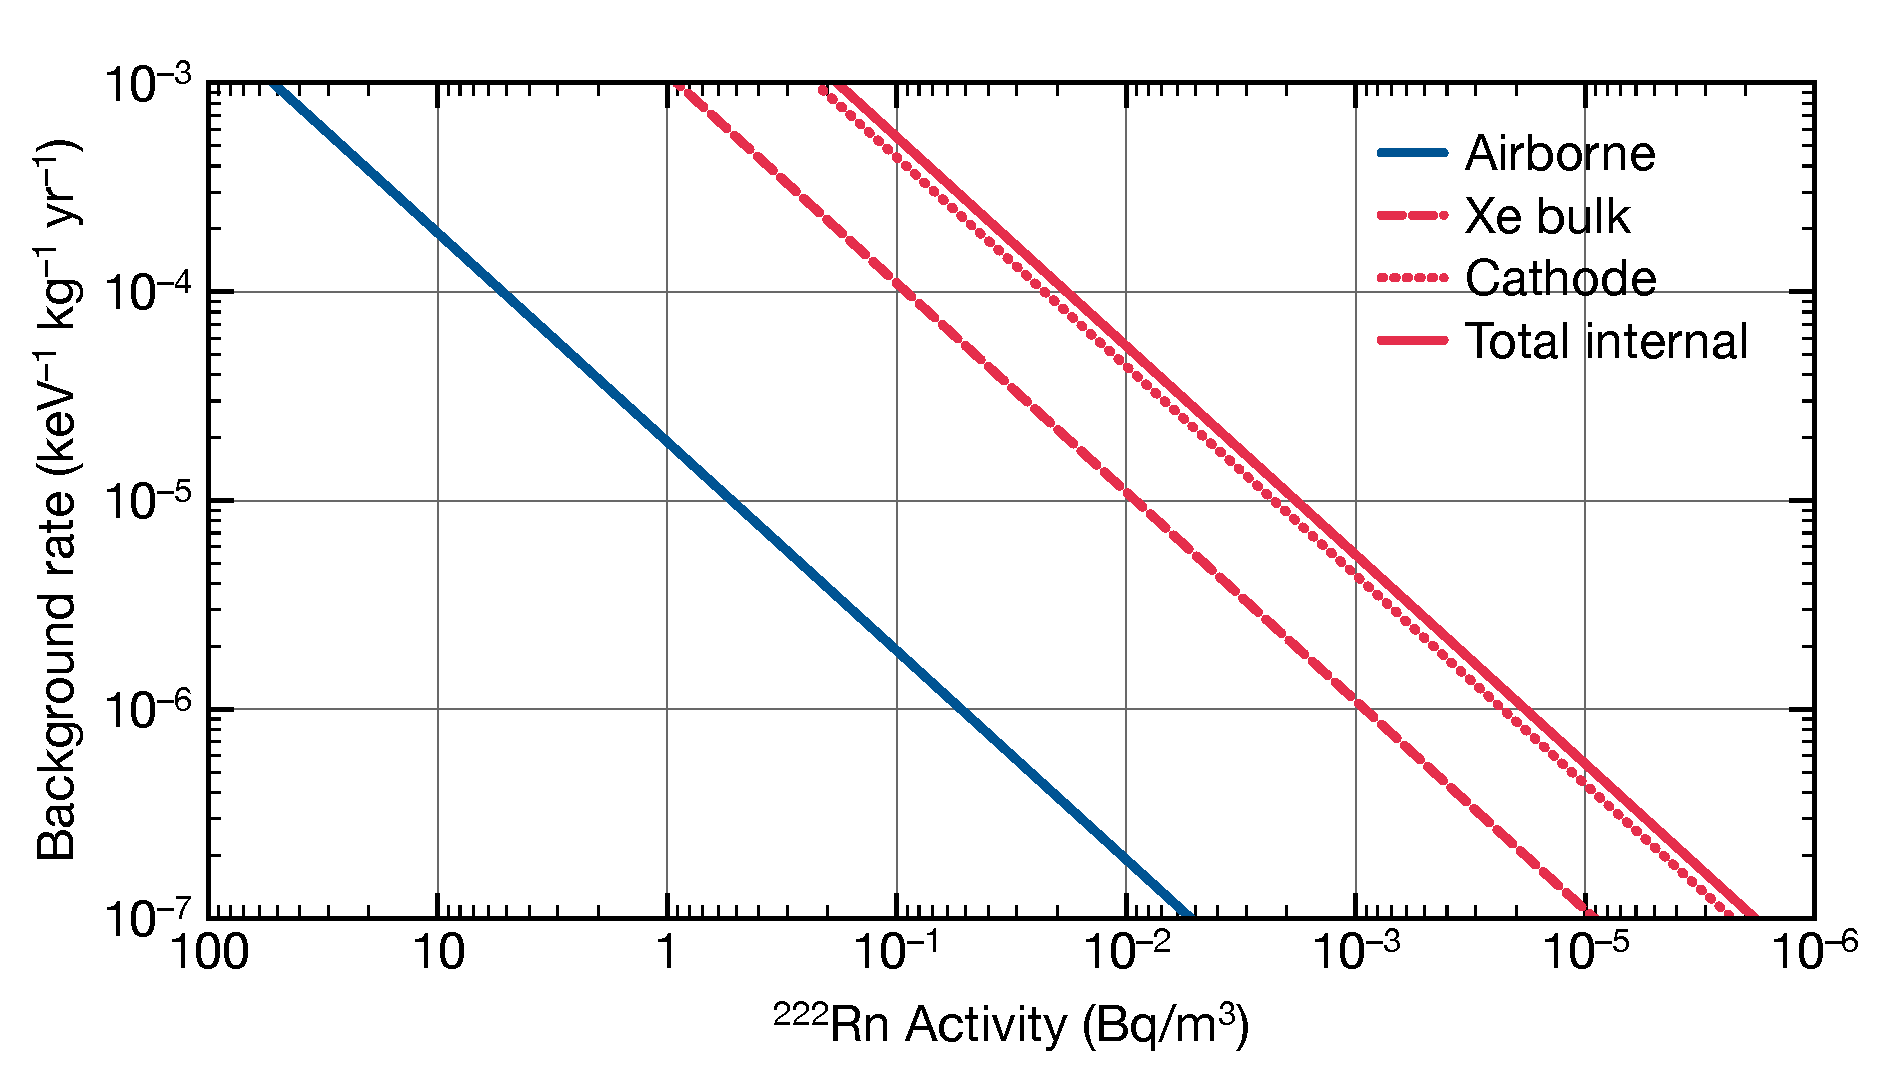
\includegraphics[width=0.9\textwidth]{img2/RadonNext100.pdf}
\caption{Background rate induced in NEXT-100 by airborne radon and radon contamination in the xenon gas (labelled as \emph{internal}) in terms of the activity of $^{222}$Rn.} \label{fig:RadonNext100}
\end{figure}
%%%%%%%%%%


Table~\ref{tab:BkgRateSummary} shows the contributions grouped into six major subsystems. The background from \Bi\ is 4.3 times more abundant than the background from \Tl. The overall background rate estimated for NEXT-100 is
%%%
\begin{equation}
<5.86\times10^{-4}~\mathrm{counts/(keV~kg~year)}\,.
\end{equation}
%%%
This rate includes only radioactive backgrounds from detector materials and components. All other sources of background are expected to contribute at the level of $10^{-5}$~keV$^{-1}$~kg$^{-1}$~yr$^{-1}$ or below:
%%%
\begin{itemize}
\item The activity of airborne radon in the vicinity of the detector --- which translates, ultimately, into \Bi\ activity on the internal surface of the lead shield and on the external surface of the vessel--- will be reduced  by at least two orders of magnitude with respect to the activity in the experimental hall of LSC ($\sim$80~Bq/m$^{3}$) thanks to the use of a radon mitigation machine or the removal of the air inside the lead shield (3.2~m$^{3}$) with clean nitrogen. The computed rejection factor for this source of background is $2\times10^{9}$, resulting in a background rate of about $10^{-5}$~keV$^{-1}$~kg$^{-1}$~yr$^{-1}$ for a $^{222}$Rn activity of 0.5~Bq/m$^{3}$ (see Figure~\ref{fig:RadonNext100} for other values of the specific activity of $^{222}$Rn in the range between 10$^{-2}$ and 10$^{2}$~Bq/m$^{3}$).
%
\item Radon contamination in the xenon gas causes two different types of background events: $\beta$ tracks from the decay of \Bi\ in the active volume, and photoelectrons generated by gamma rays emitted, for the most part, from the TPC cathode following the decay of \Bi. In the EXO-200 TPC, the latter type of events constitute about 80\% of the measured activity of $^{222}$Rn in the liquid xenon, while the former make up the remaining 20\% \cite{Albert:2013gpz}. The rejection power against both types of background events is similar, approximately $2.5\times10^{6}$. In the case of the $\beta$ decays of \Bi\ in the xenon bulk, we have assumed that Bi-Po tagging --- i.e.\ the coincident detection in an event of the $\beta$ emitted in the decay of \Bi\ and the alpha emitted by $^{214}$Po shortly after--- can be done with high efficiency ($\gtrsim99\%$). Figure~\ref{fig:RadonNext100} (red lines) shows the background rate generated in NEXT-100 by this internal contamination of radon in terms of the activity of $^{222}$Rn. In order for this background to contribute, at most, at the level of $10^{-5}$~keV$^{-1}$~kg$^{-1}$~yr$^{-1}$, radon activities in the xenon gas below a few mBq per cubic metre will be required. The EXO-200 detector, which has been operating without a radon suppression system, has measured, for instance, an activity of $^{222}$Rn of that order in their xenon volume: $(3.65\pm0.37)~\mu\mathrm{Bq/kg}$ \cite{Albert:2013gpz}. Similarly, the radon activity of the NEMO-3 tracking gas was measured to be about 5~mBq/m$^{3}$ \cite{Arnold:2013dha}.
%
\item Out of the 50 atoms of $^{137}$Xe produced on average every year by neutron activation of \Xe\ (\textsection~\ref{subsec:MuonsNeutrons}), 0.25 of them will decay emitting a $\beta$ track with energy within our region of interest. These events will be suppressed by about a factor of 10 by the 2-blobs selection criterion, yielding a background rate of approximately $9\times10^{-6}$~keV$^{-1}$~kg$^{-1}$~yr$^{-1}$. Nevertheless, the neutron flux can be attenuated by several orders of magnitude using polyethylene shielding of a few tens of centimetres in thickness.
\end{itemize}
%%%








%%%%%%%%%%%%%%%%%%%%%%%%%%%%%%%%%%%%%%%%%%%%%%%%%%%%%%%%%%%%
\subsection{Sensitivity of NEXT-100}
%%%
The sensitivity of NEXT-100 to neutrinoless double beta decay --- calculated following the Feldman-Cousins prescription for the construction of confidence intervals \cite{Feldman:1997qc, GomezCadenas:2010gs} --- is shown in Figure~\ref{fig:SensitivityNEXT100}. In the top panel, the sensitivity (at 90\% CL) to the half-life (red, solid curve) and the corresponding sensitivity to \mbb\ (blue, dashed curves) for the largest and smallest nuclear matrix element calculations published (e.g, the ISM model predicts an NME of 2.19 \cite{Menendez:2008jp} 
while  \cite{Yao:2014uta} finds a value of 4.32 using the EDF model). 
are represented in terms of the exposure, assuming a signal detection efficiency of 28\% and a background rate of $6\times10^{-4}~\ckky$. The bottom panel shows, for an exposure of 100~kg$\cdot$year the variation of the sensitivity with respect to the background rate in the range between $10^{-5}$ and $10^{-4}$~\ckky.


%%%%%%%%%%
\begin{figure}
\centering
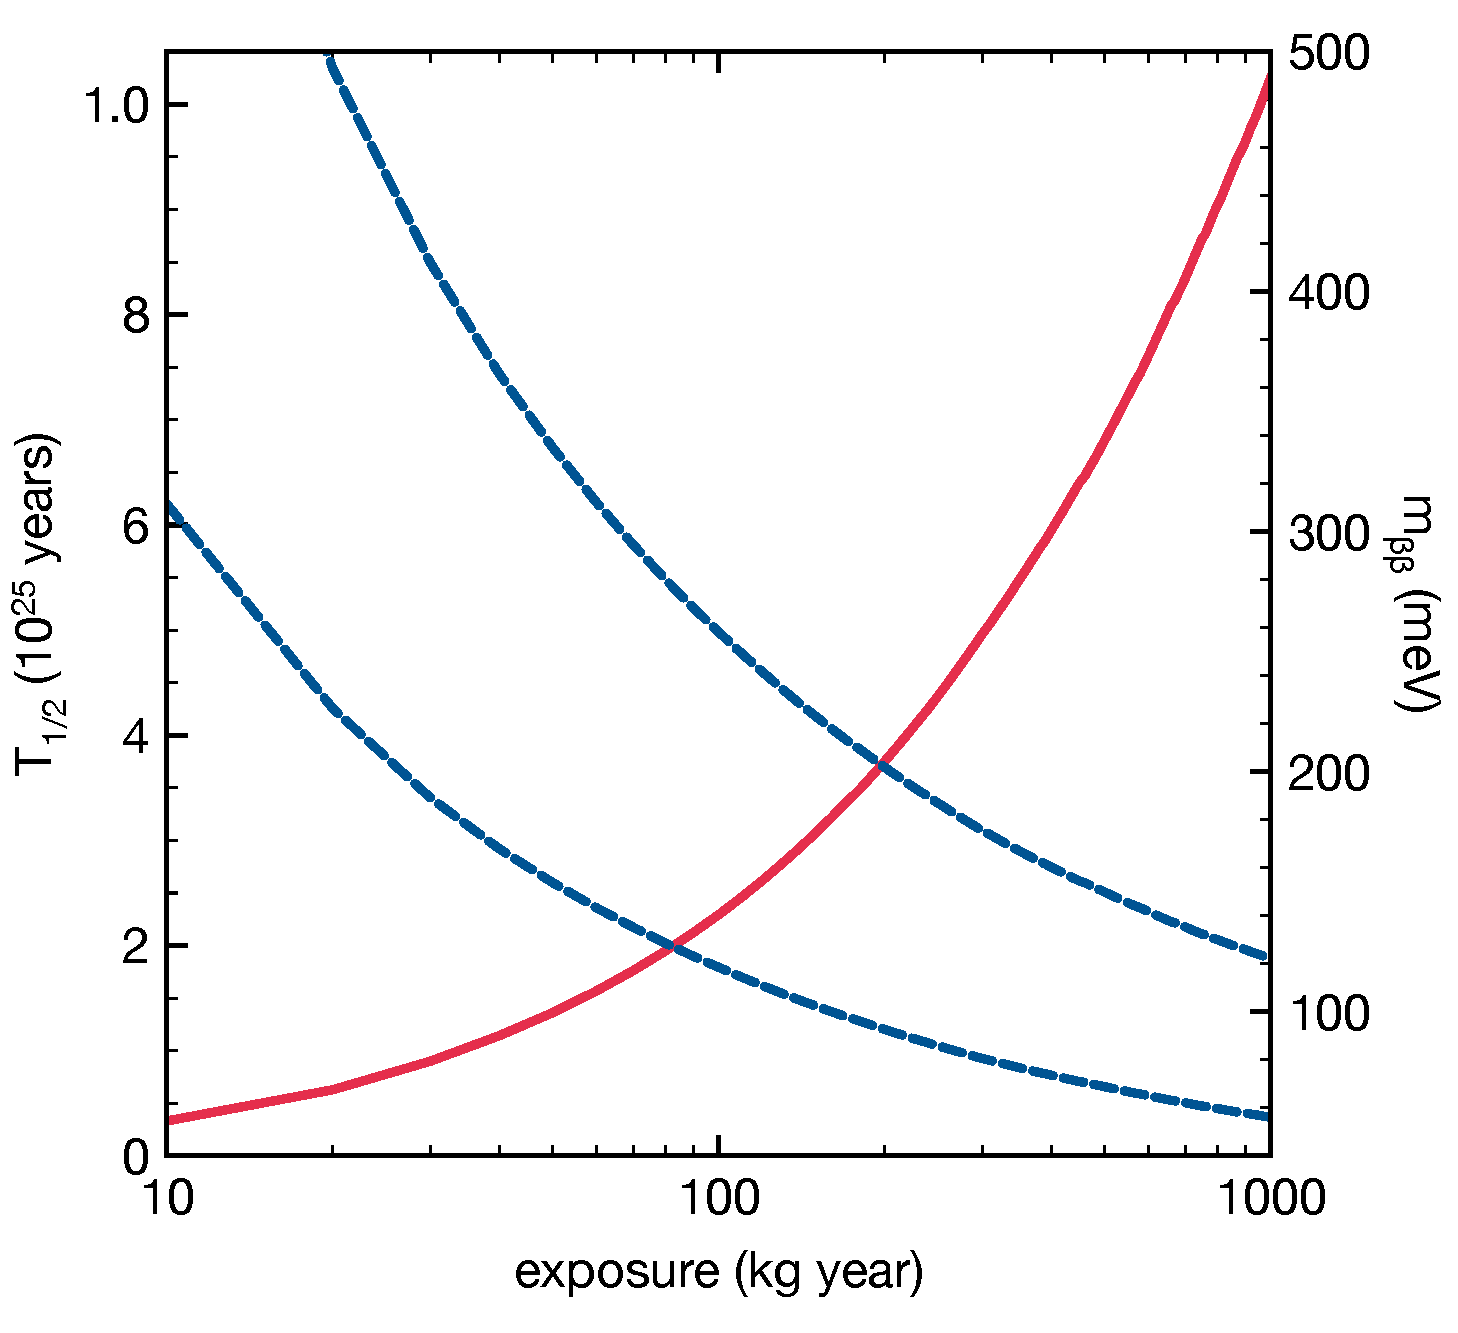
\includegraphics[width=0.7\textwidth]{img2/Next100SensitivityVsExposure.pdf}
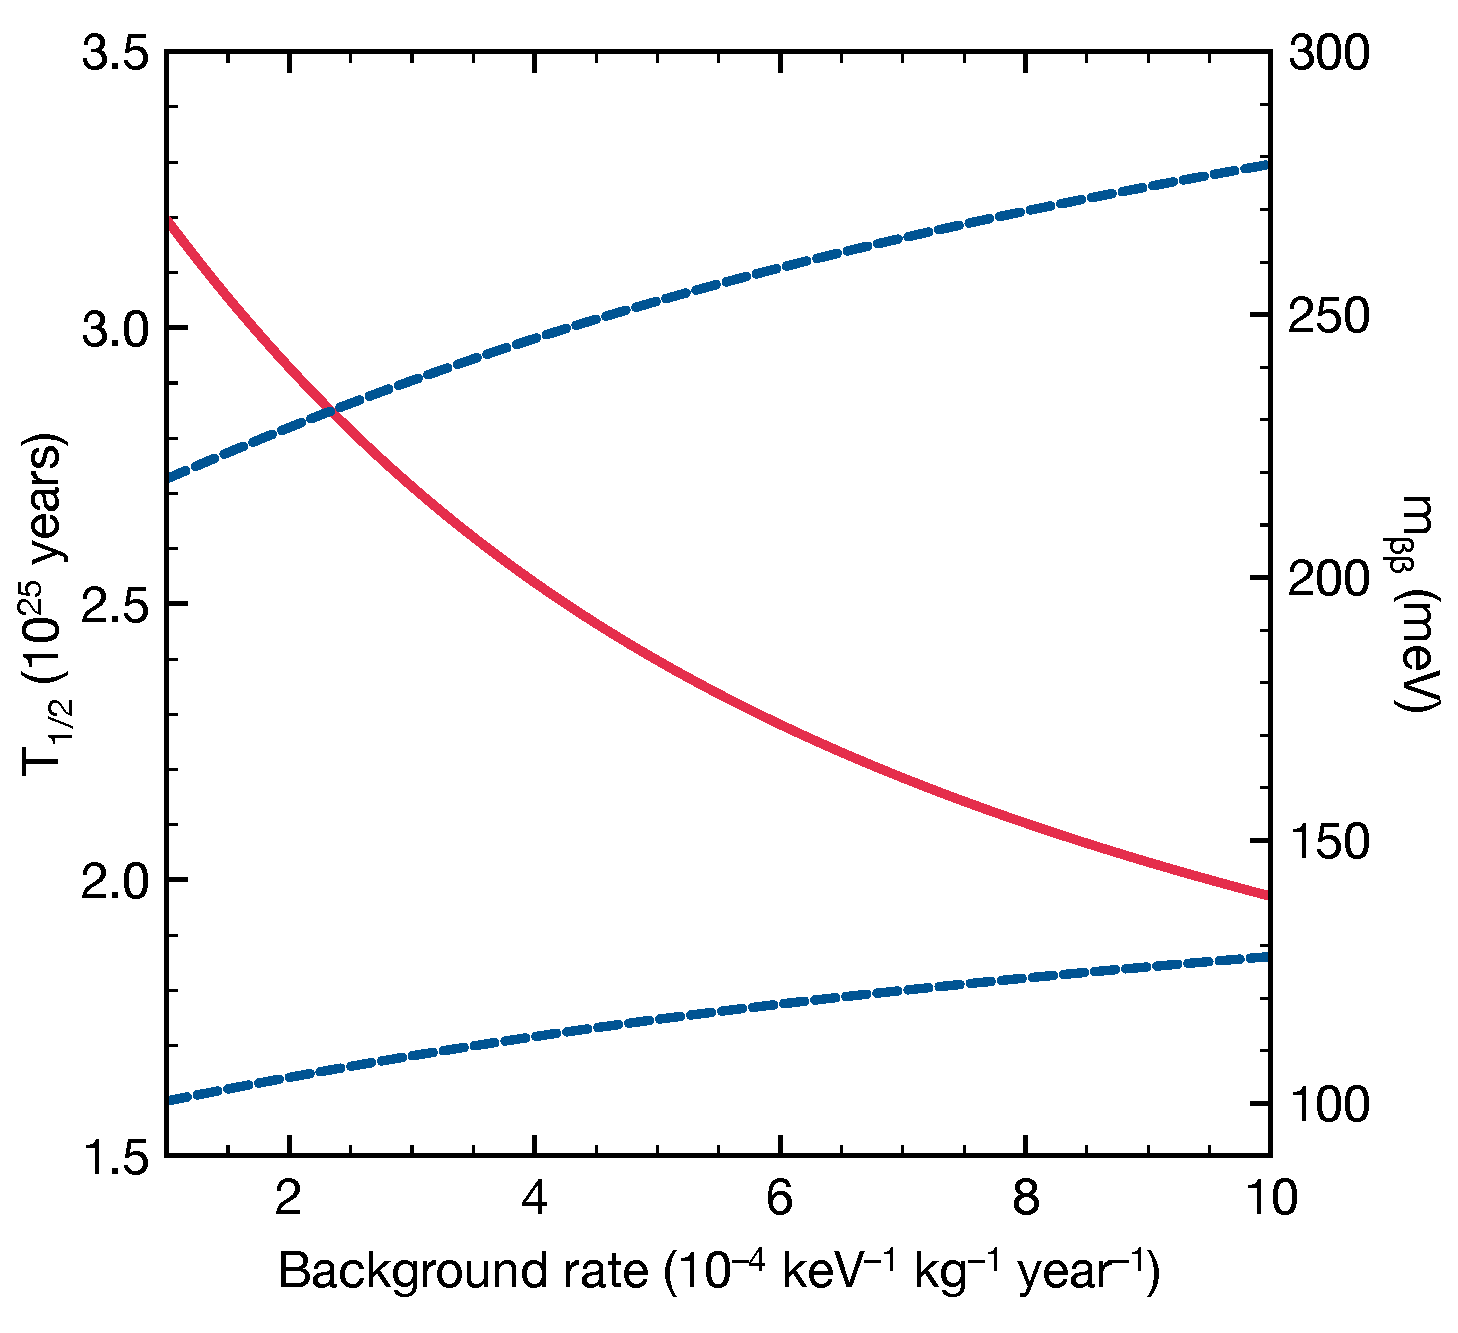
\includegraphics[width=0.7\textwidth]{img2/Next100SensitivityVsBackground.pdf}
\caption{Sensitivity of NEXT-100 to neutrinoless double beta decay. Top: Sensitivity (at 90\% CL) to the \bbonu-decay half-life (red. solid curve) and the corresponding \mbb\ sensitivity (blue, dashed curves) for the largest and smallest NME calculations in terms of the exposure. Bottom: Sensitivity (at 90\% CL) in terms of the background rate.} \label{fig:SensitivityNEXT100}
\end{figure}
%%%%%%%%%%


\section{\label{sec.new}The NEW detector}


%%%%%%%%%%
\begin{figure}
\centering
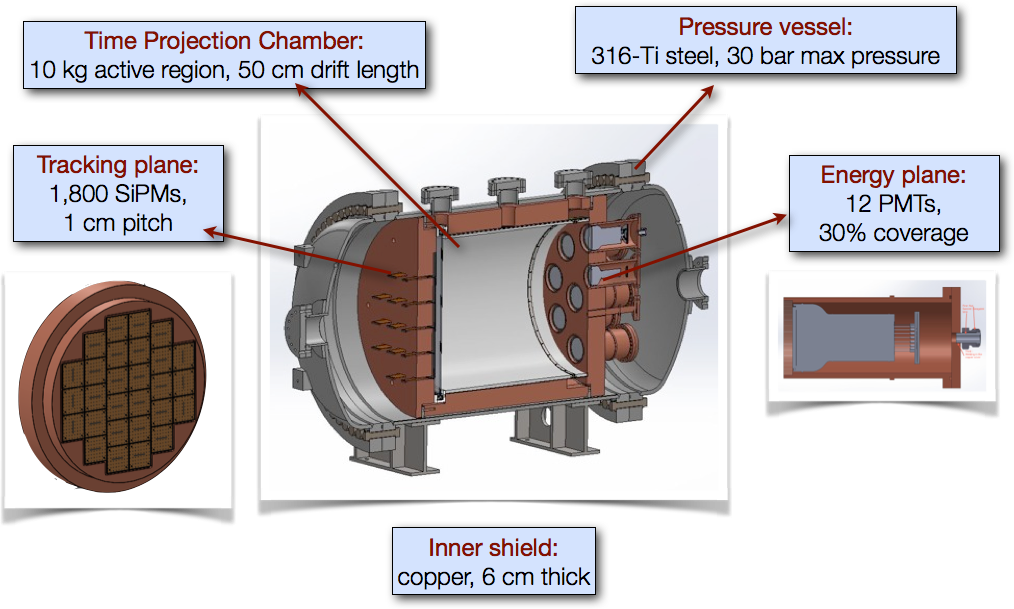
\includegraphics[width=0.9\textwidth]{img2/NEW.png}
\caption{\small The NEW apparatus.} \label{fig:NEW}
\end{figure} 

%%%%%%%%%%
\begin{figure}
\centering
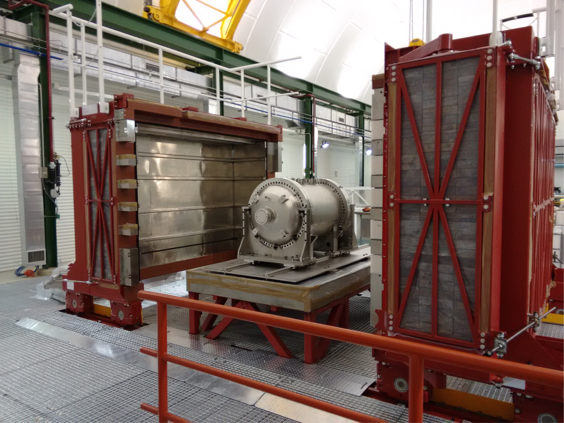
\includegraphics[width=0.9\textwidth]{img2/NewCastle.png}
\caption{\small The NEW detector, sitting inside the Lead Castle at the Canfranc Underground Laboratory.} \label{fig.NewCastle}
\end{figure} 

%\begin{figure}
%\centering
%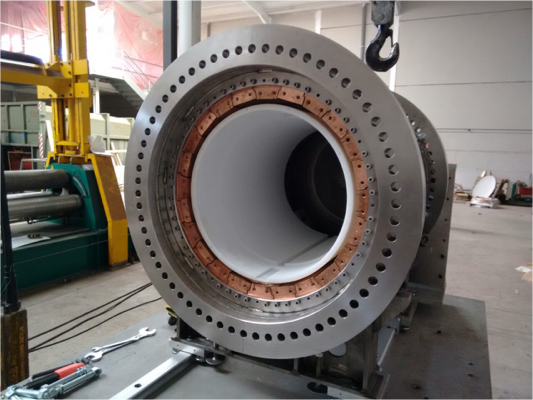
\includegraphics[width=0.9\textwidth]{img2/NewICS.png}
%\caption{\small The NEW detector, showing the inner copper shield (ICS), 6 cm thick and the outer frame of the field cage.} \label{fig.NewICS}
%\end{figure} 

\begin{figure}
\centering
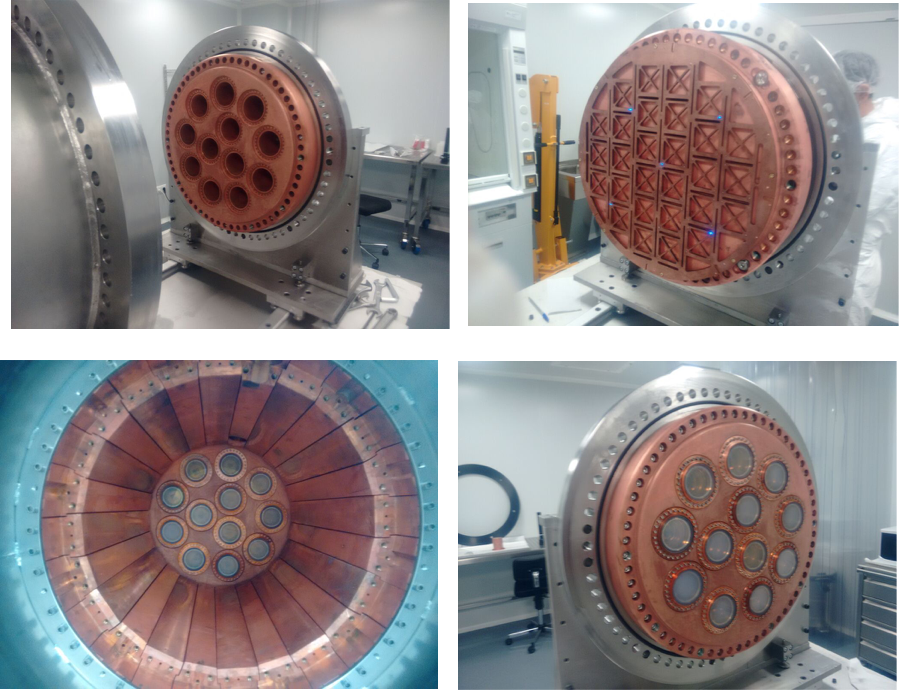
\includegraphics[width=0.9\textwidth]{img2/EP.png}
\caption{\small Top left: energy plane support; top right: tracking place
support; bottom left: energy plane installed inside NEW, with the PMTs in place; 
top right; energy plane displaying the sapphire windows, coated with TPB.} \label{fig.EP}
\end{figure} 


\begin{figure}
\centering
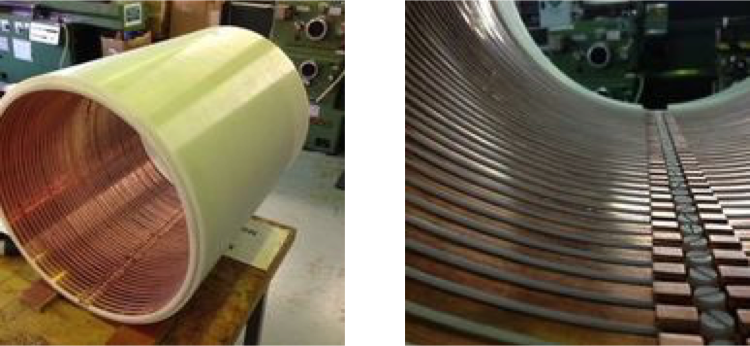
\includegraphics[width=0.9\textwidth]{img2/FieldCage.png}
\caption{\small The NEW field cage mounts copper rings connected by radiopure resistors in a cylindrical body of high density polyethylene. The field cage has 0.5 m diameter and 0.5 m length.} \label{fig.FC}
\end{figure}


The NEW (NEXT-WHITE) apparatus\footnote{The name honours the memory of the late Professor James White, one of the key scientists of the NEXT Collaboration.}, shown in Figure \ref{fig:NEW}, is the first phase of the NEXT detector to operate underground (Figure \ref{fig.NewCastle}). NEW 
is a scale 1:2 in size (1:8 in mass) of NEXT-100. The energy plane contains 12 PMTs (20 \% of the 60 PMTs deployed in NEXT-100, see Figure \ref{fig.EP}). The tracking plane technology consists of 30 Kapton Dice Boards (KDB) deploying 1800 SiPMs (also 20\% of the sensors). The field cage has a diameter of 50~cm and a length of 50~cm (Figure \ref{fig.FC}). 

NEW is a major step for the NEXT project, and will allow us to address a number of crucial questions. Specifically:

\begin{enumerate}
\item {\bf Energy resolution}: the aspect ratio of NEW is the same to that of NEXT-100 (and DBDM, but better than DEMO). The larger dimensions of the detector allow to contain large tracks and therefore to include in the study energetic sources. This will permit a study of the resolution at 511 keV and 1.2 MeV (\NA\ source), 660 keV (\CS\ source), 1.5 MeV and 2.6 MeV (\THO\ source). 
\item {\bf Topological signature}: we will repeat the analysis that we have just carried out in DEMO, using 511 keV, 660 keV, 1.2 MeV and 2.6 MeV single electrons (from \NA, \CS\ and \THO\ sources) as well as double electrons from the \TL\ double escape peak to understand with detail the efficiency and rejection power of the topological signature. 
\item {\bf Background model:} Comparison of data and Monte Carlo should help us to validate our background model (currently based exclusively in Monte Carlo calculations) and to identify and correct possible hot spots.
 \item {\bf Impact of radon:} In 2016 NEW will operate inside a radon-free tent (the infrastructure has been approved by the LSC and in currently being ordered to the vendor). Analysis of our data and Monte Carlo comparison should permit the quantification of the effect of radon degassing inside the detector.
 \end{enumerate}

In addition, NEW will allow us to quantify any potential technical issues. Among these:
 
 \begin{enumerate}
\item {\bf S1 and S2 signals}: We will measure the number of photoelectrons for S1 and S2 signals produced near \Qbb\, in order to ensure that photoelectron statistics does not degrade the energy resolution. The effect of sapphire windows and TPB coating in light collection will be evaluated (DEMO used bare PMTs sensitive to VUV and very radioactive).  
\item {\bf Electron lifetime}: DEMO achieved electron lifetimes in excess of 10 ms. The same or better should be achieved with NEW. A much better measurement can be made here, given the long drift in NEW field cage. 
\item {\bf Operational stability and sparks:} In DEMO the frequency of sparks was of the order of one a week. NEW uses a quartz plate coated with ITO in the region facing the SiPMs. Sparks should be rare, but its frequency and effect (e.g, in the TPB coating the plate) must be measured. 
 \item {\bf Leaks:} The energy plane is separated from the main volume defined by the field cage by a plate sealing the PMTs, which operate in vacuum. The PMTs are coupled to the main volume by sapphire windows. The system needs to operate without leaks between the main volume in the energy plane for long periods of time.
 \end{enumerate}

Other important issues where NEW will allow steady progress are:

 \begin{enumerate}
\item {\bf Gas system}, which is the same that will be used for NEW-100. In particular, NEW will test for more than one year the state-of-the-art, triple-metal-sealing compressor manufactured by the German company SERA for NEXT, before operation with enriched xenon. 
\item {\bf FEE, DAQ and SC}: The front-end electronics of the PMTs and SiPMs, the DAQ system and the slow controls are identical for NEW and NEXT-100, and operation of the former will allow to spot and correct any unforeseen issues. 
 \end{enumerate}
 


\section{Towards a ton-scale high-pressure xenon TPC.}
\label{sec.ts}


%%%%%%
\begin{figure}
\centering
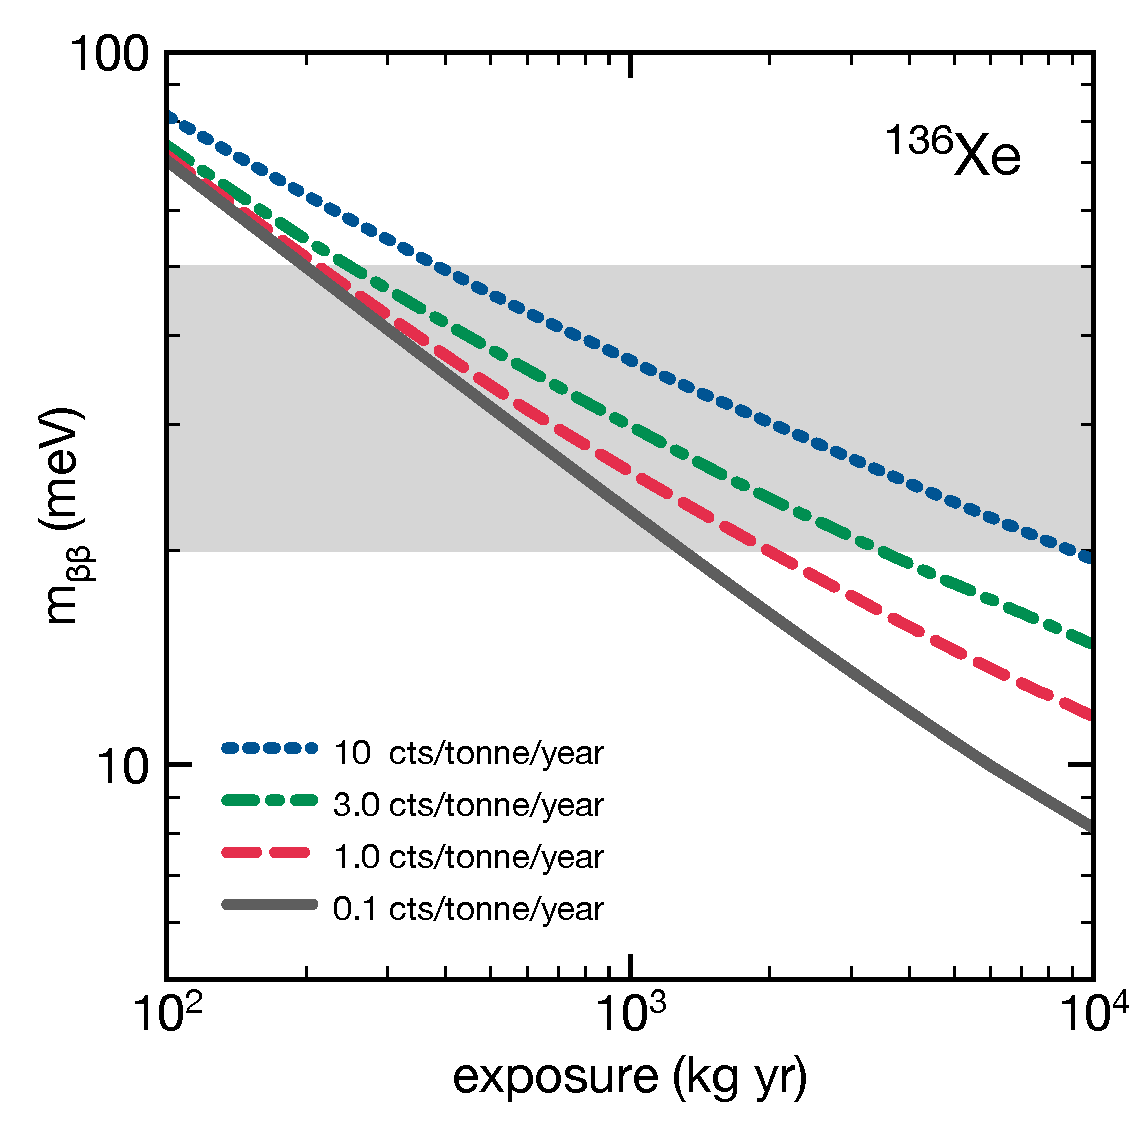
\includegraphics[width=0.90\textwidth]{img2/FutureXe136.pdf}
\caption{\small Sensitivity to \mbb\ as a function of the exposure for different values of the background, for a \XE\ based experiment.} \label{fig.Xe}
\end{figure}
%%%%%%

If no discovery is made by the current generation of experiments, the full exploration of the inverse hierarchy (IH) region (corresponding to \mbb\ values as low as 15~meV) requires detectors of larger mass (at least 1 ton), good resolution and extremely low specific background. In this section we discuss the capabilities of the \HPXE\ technology to explore this scale. 

\subsection{NEXT/NEW as R\&D for a future ton-scale HPXe}

The first goal of the NEXT collaboration during the next three years is to demonstrate, first with NEW, then with NEXT-100, the excellent energy resolution, topological signature and low radioactive budget describe in previous sections. 

It is worth to consider the potential of the HPXe technology using the projected NEXT-100 figures. For a background rate of $6 \times 10^{-4}$ \ckky and an energy resolution of 0.5\% FWHM (e.g, a ROI of 12.5 keV), NEXT would record $\sim$8 events per ton and per year. Naive scaling arguments suggest an improvement of a factor $\sim$2 in the background as the detector dimensions double (and the detector mass multiplies by $\sim$8) to build a ton-scale apparatus. Thus, 4 counts per ton and per year could be expected by a direct extrapolation of the NEXT-100 expected performance. According to Figure \ref{fig.Xe} it would require an exposure of $3 \times 10^{3}~kg\cdot year$, for a 100\% efficient detector, to fully cover the IH. The efficiency of NEXT is around 30\%, and thus, about 10 (5) years of data taking would be necessary to explore the IH for a 1 (2) ton detector which were a direct extrapolation of NEXT-100 (no technological improvement). This qualifies the HPXe technology as a candidate for the ton scale, (since it can cover the IH in a credible time deploying a credible fiducial mass), {\em using existing technology}, provided that NEXT-100 demonstrates both an
energy resolution in the vicinity of 0.5\% FWHM at \Qbb\ and a background rate in the range of 
$5-6 \times 10^{-4}$ \ckky. Thus, NEXT-100, in addition of its physics interest (it can explore a region of effective Majorana masses in the vicinity of $\mbb \sim 100$meV, where a discovery is still possible) can be considered a demonstrator and R\&D apparatus for a ton-scale HPXe-EL.

\subsection{Improving the rejection power of the topological signature}

%%%%%%
\begin{figure}
\centering
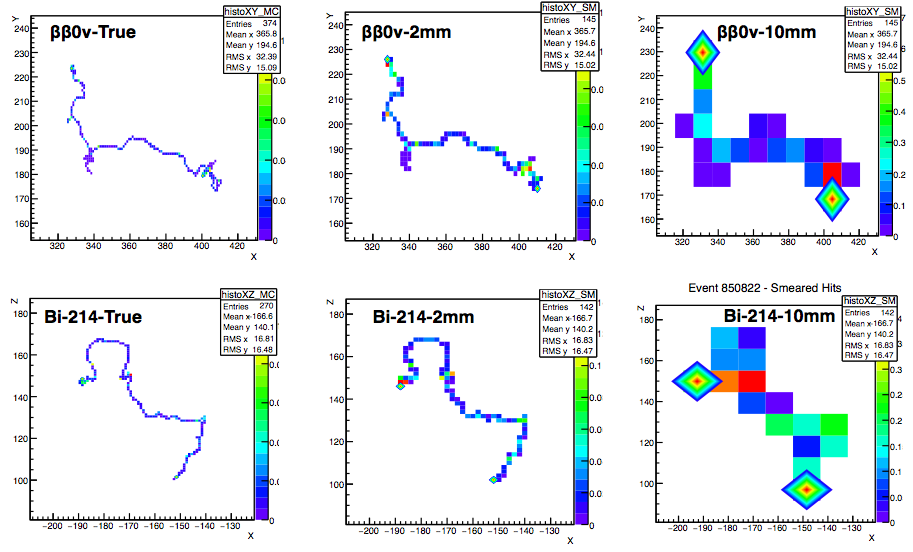
\includegraphics[width=0.90\textwidth]{img2/tracks.png}
\caption{\small Top left: Monte Carlo true hits left by a \bbonu\ event in
an HPXe with no diffusion; top center: hits corresponding to a diffusion of
$2 mm/\sqrt{E}$; top right: hits corresponding to a diffusion of
$10 mm/\sqrt{E}$. Bottom: same, for a single electron produced
by \BI\ decay.} \label{fig.trks}
\end{figure}
%%%%%%

On the other hand, we believe that the performance of an HPXe-EL TPC can improve significantly {\em by improving the topological signature}. 

Currently, the discriminating power of the topological signature is limited by the large diffusion unavoidable in pure xenon. Such large diffusion, of the order of $10 mm/\sqrt{1 m}$, has the effect of blurring the electron(s) trajectory. This, in turn, makes more challenging the task of connecting the hits making up the track and identifying its extremes, where the algorithm searches for the blobs. 

This is illustrated in Figure \ref{fig.trks}. The top panels show a \bbonu\ event, while the bottom panels show a single electron produced by \BI\ decay. From left to right, one can see the true hits of the tracks, and the hits corresponding to a diffusion of $2 mm/\sqrt{E}$~and to a diffusion of
$10 mm/\sqrt{E}$. Notice that in the late case the details of the track are blurred, and in fact, the reconstruction algorithm misidentifies a second blob in the background event, while it succeeds in finding a single blob for the lower diffusion case. 

%%%%%%
\begin{figure}
\centering
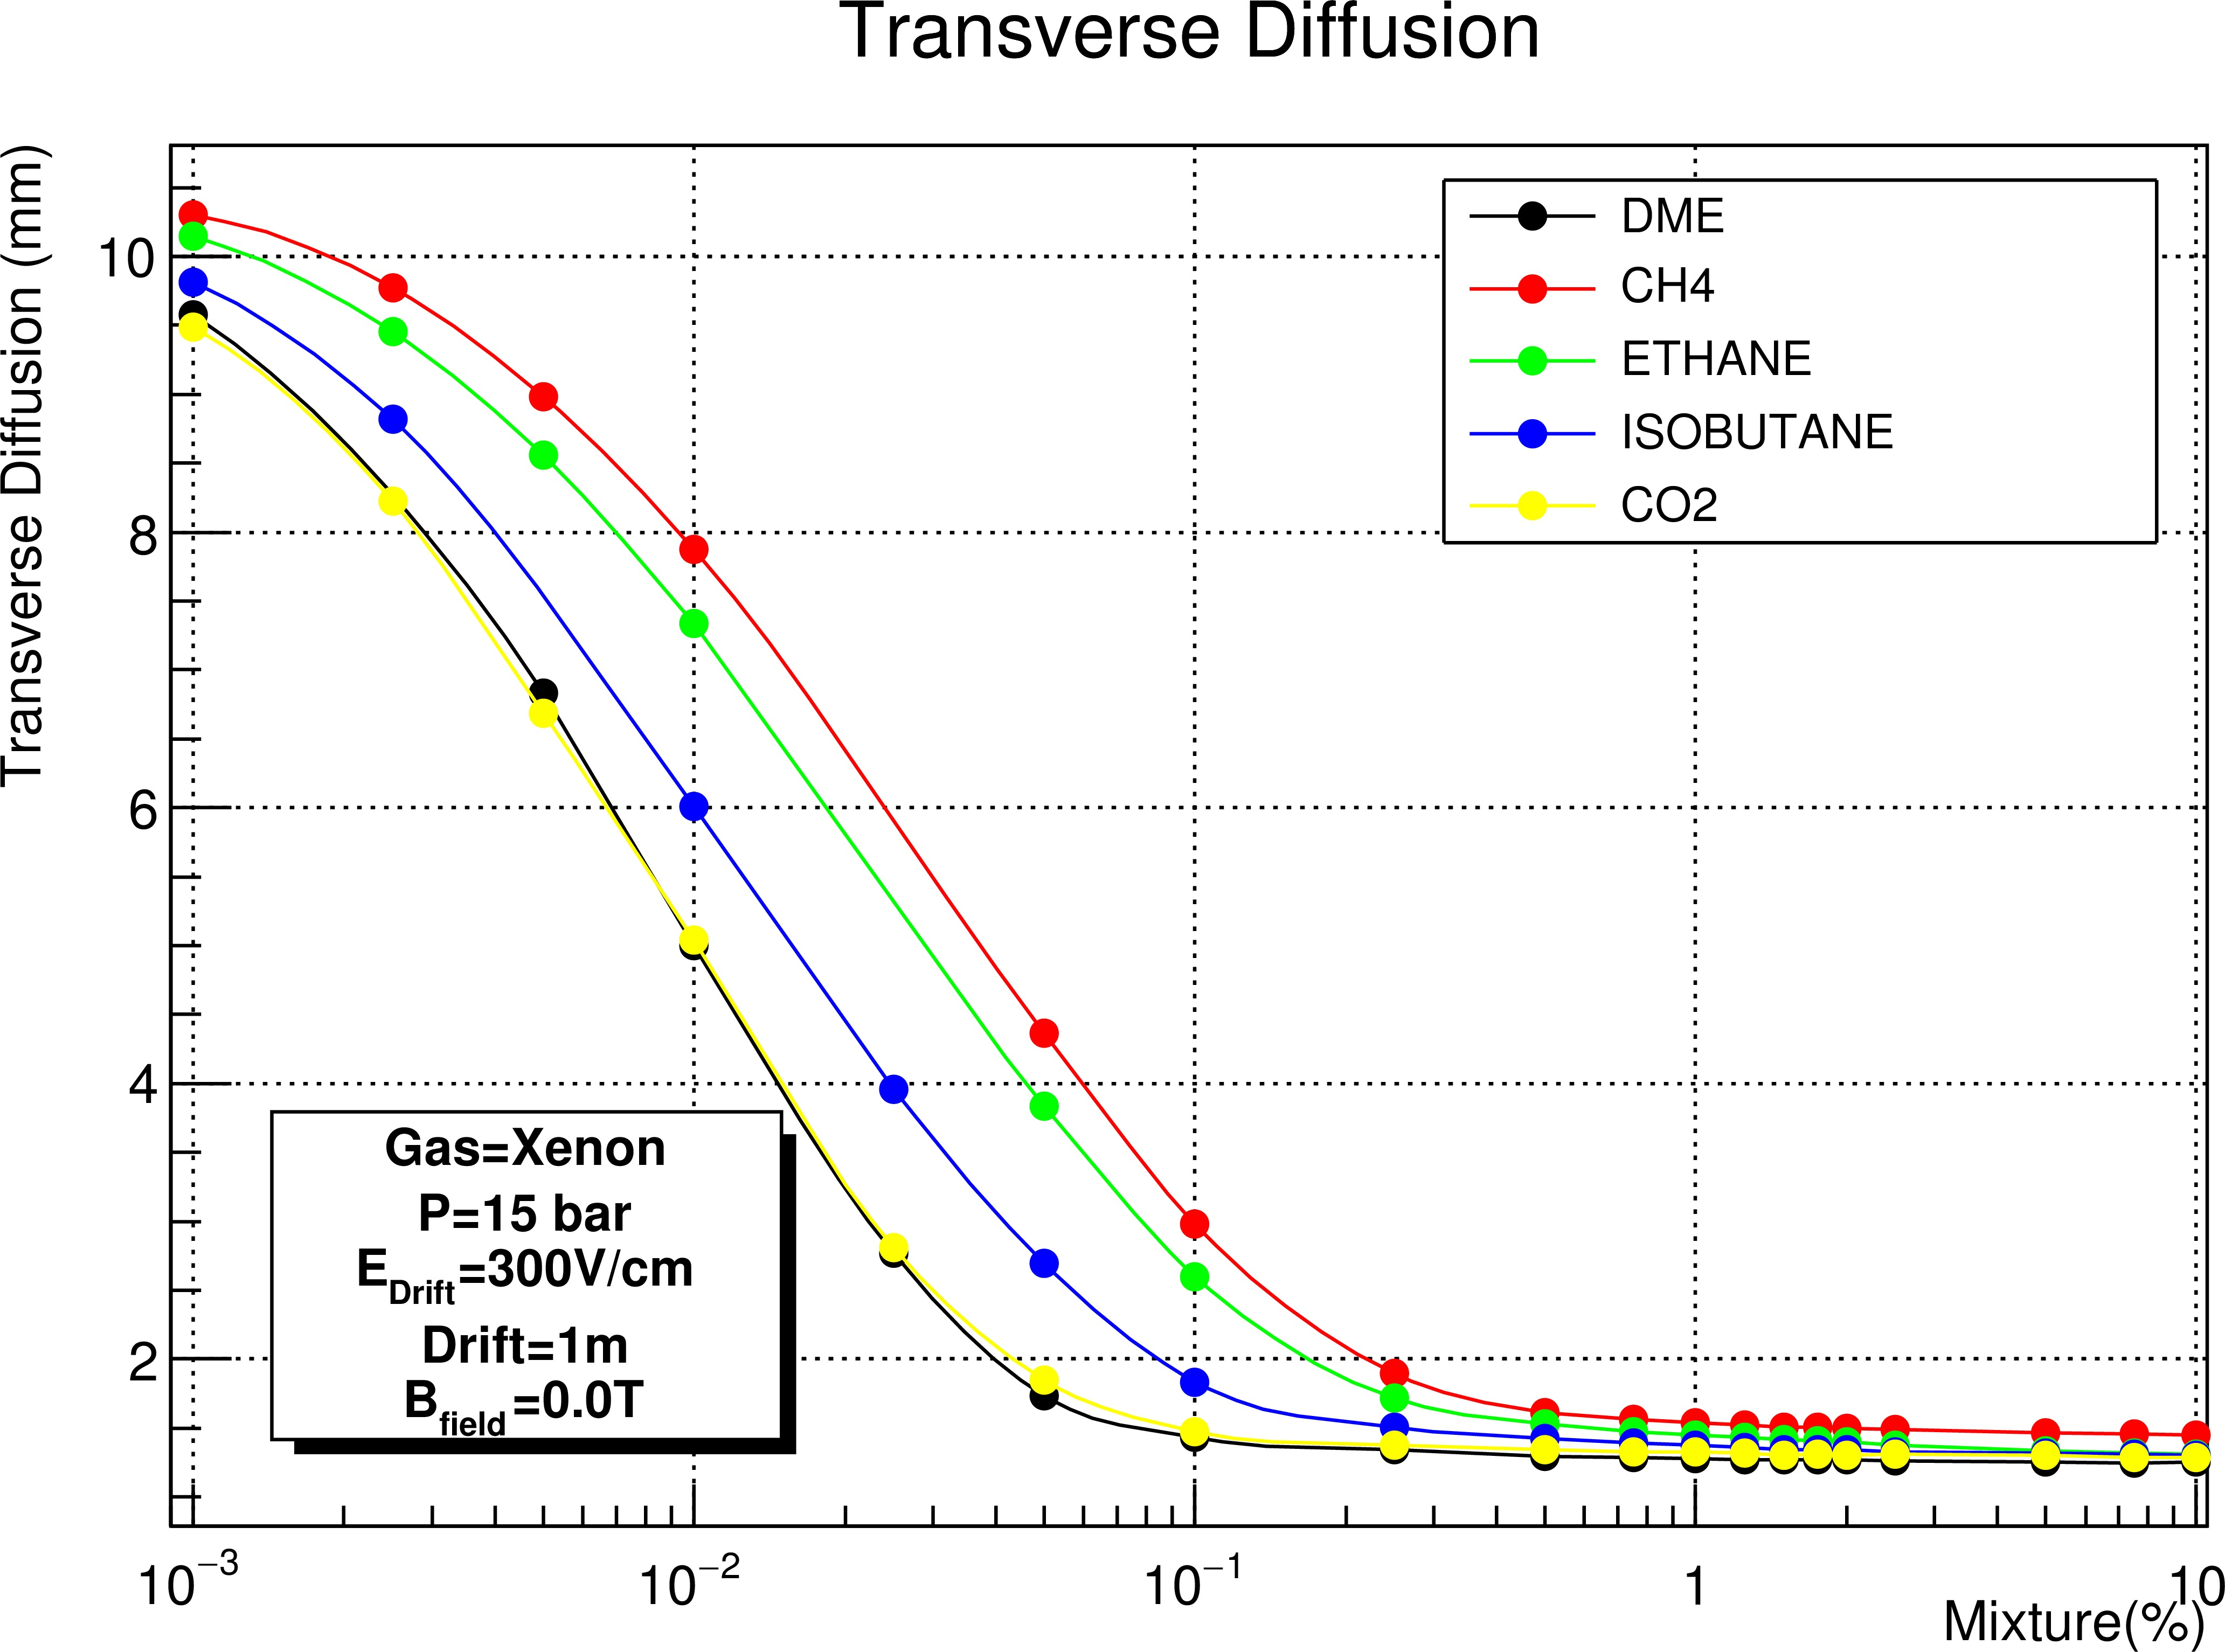
\includegraphics[width=0.90\textwidth]{img2/TD300V.jpg}
\caption{\small Adding small quantities of quencher gases can reduce the diffusion of Xenon to $\sim 1 mm/\sqrt{1 m}$.} \label{fig.QG}
\end{figure}
%%%%%%

%%%%%
%\begin{figure}[!htb]
%	\centering
%	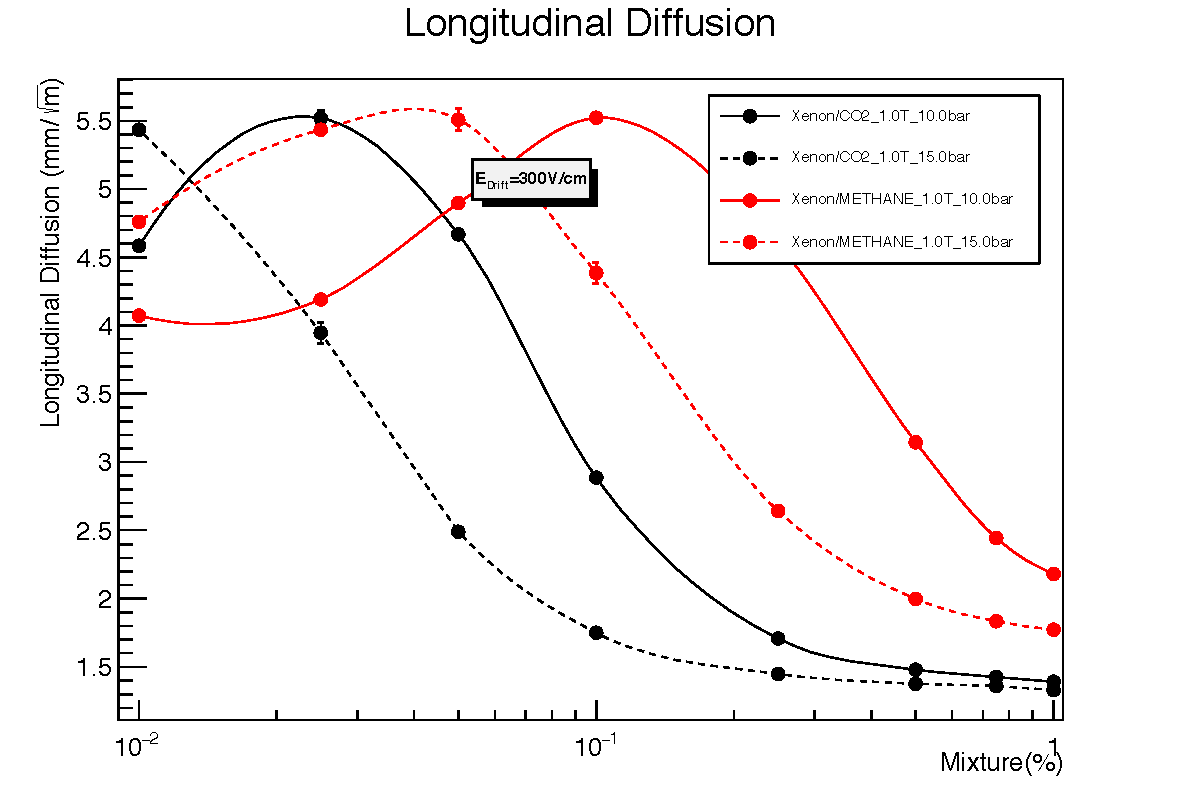
\includegraphics[width=0.75\textwidth]{img/Longitudinal_Diffusion300Vcm.pdf}
%	\includegraphics[width=0.75\textwidth]{img/Transverse_Diffusion300Vcm.pdf}
%	\caption{\label{fig.QG}Longitudinal and transverse diffusion when small amounts of \COT\ and \CHF\ are added to pure xenon. Notice that about 0.3 \% of \COT\ are enough to reduce both longitudinal and transverse diffusion to about $1.5$~mm/$\sqrt{\rm{m}}$.}
%\end{figure}
%%%%%


%%%%%%
\begin{figure}
\centering
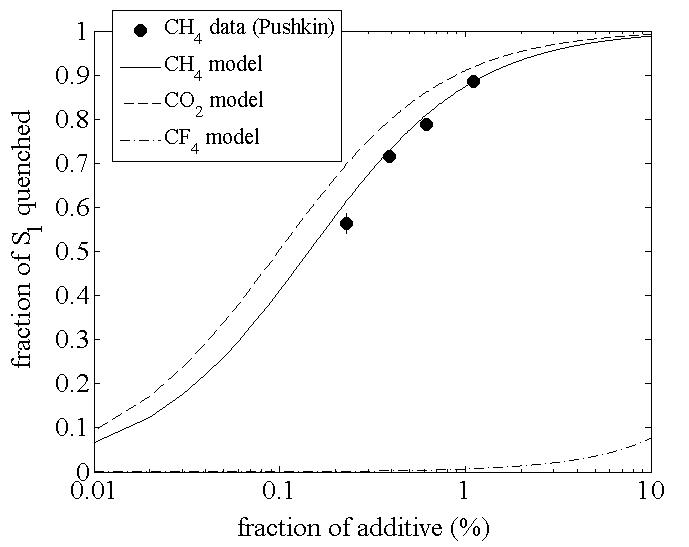
\includegraphics[width=0.90\textwidth]{img2/QF.png}
\caption{\small Adding small quantities of quencher gases also reduces the scintillation light. The plot shows the fraction of S1 light quenched as a function of the fraction of gas added. Notice that a fraction of 0.1\% (0.5\%) of \COT (\CHF) quenches the S1 signal by about 50\% } \label{fig.QF}
\end{figure}
%%%%%%

Diffusion in xenon can be reduced to values as small as 1 mm by adding small amounts of quenching gases, as illustrated in Figure \ref{fig.QG}. On the other hand, quencher gases are known to reduce significantly or even suppress the xenon scintillation light in sufficiently large amounts, as illustrated in Figure \ref{fig.QF}. A major R\&D for the NEXT collaboration during the forthcoming period is to explore the performance of the detector when adding small  mixtures of gases such as \COT\ or \CHF. For example, adding 0.1\% (0.5\%) of \COT (\CHF) would reduce the diffusion to some 2 mm over 1 m of drift, while the predicted quenching of the light would be about 50\%, a factor that appears tolerable and can be partially compensated with higher EL amplification and/or better light collection. 

The R\&D program of NEXT concerning reduction of the diffusion for the next 3 years include:
 \begin{enumerate}
\item {\bf Study of gas mixtures with small setups}. This is already under way, with interesting initial results that suggest that quenching can be smaller than predicted by Monte Carlo calculation. One has to understand carefully, however, the systematics of the measurements. The goal of this studies is to focus in one or two candidates that can be further explored in larger setups. Both \COT\ and \CHF\ appear promising. 
\item {\bf Study of performance in DEMO}. We expect to start the study of selected mixtures (e.g, xenon + 0.1\% \COT, xenon + 0.5\% \CHF) in the NEXT-DEMO detector, late in 2015. DEMO is capable of measuring both S1 and S2 signals, and reconstruct electron tracks, and should provide a quantitative assessment of the effect of the selected mixtures in aspects such as reduction of diffusion, quenching of S1 and S2, attachment, and energy resolution. The goal of the campaign in DEMO is to identify one suitable gas mixture for further studies.
\item {\bf Study of performance in NEW}. Assuming that the previous studies yield promising enough results, the suitable gas mixture candidate(s) will be studied in NEXT during 2017 (2016 will be devote to a run with pure xenon). 
\end{enumerate}

Reducing diffusion to $\sim 2 mm/\sqrt{1 m}$, improves the background rejection of the
HPXE-EL automatically, since the algorithm that finds the blobs at the extremes of the track works much better with the considerable improvement in the hit resolution. Indeed, out Monte Carlo calculations show an improvement of a factor 3-4 in the topological signal rejection factor by simply reducing diffusion to  $\sim 2 mm/\sqrt{1 m}$. This, in turn, translates into 2-3 counts per ton and per year in NEXT-100, and 1-2 counts per ton and per year in a ton scale detector. 
{\em It follows that reducing the diffusion in pure xenon to a target value of 2 mm for 1 m drift while maintaining the energy resolution would permit the exploration of the IH in a short time (e.g, 3 years run) with a HPXE-el of moderate mass (1 ton).}  


\subsection{Adding a magnetic field to enhance the topological signal}
In this section we present a brief status of the on-going studies within the NEXT collaboration to explore the potential of adding a magnetic field to the detector. 

There are two conditions {\em sine qua non}, for a magnetic field to increase the rejection power of an HPXe in a significant way:

\begin{enumerate}
\item The hit resolution must be acceptably low, in the range of 1-3 mm. Thus, a pre-condition for considering the use of a magnetic field is to find a gas mixture providing  low diffusion at an acceptable cost in performance.
\item The track reconstruction must be very efficient finding the extremes of the track and following the track trajectory. This appears possible, for low diffusion (e.g, for a resolution of about 2 mm) using sophisticated pattern recognition algorithms such as minimum spanning trees followed by segment connection.  
\end{enumerate}

When both conditions are fulfilled, it is possible to ``follow'' the track trajectory from one extreme to the other and compute locally quantities such as the track curvature. Notice that the high multiple scattering in dense gas prevents event-by-event measurements of standard variables such as the momentum, or the track curvature. However, one can turn them into statistical estimators, capable of discriminating signal from backgrounds. 

In particular, if the direction of the applied magnetic field is known, the curvature of the track can be calculated to determine whether the component of the electron velocity along the magnetic field is parallel or antiparallel to the field.  Assuming that the magnetic field is directed along the z-axis, we are interested in the curvature of the track in the $x$-$y$ plane as it progresses in $z$.  The curvature $\kappa$ in the $x$-$y$ plane can be calculated for a track parameterized by the coordinate $z$ as

\begin{equation}\label{eqn_curv}
\kappa = \frac{(dx/dz)\cdot(d^2y/dz^2) - (dy/dz)\cdot(d^2x/dz^2)}{\Bigl[(dx/dz)^2 + (dy/dz)^2\Bigr]^{3/2}}.
\end{equation}

With this definition, an electron traveling in the direction of the magnetic field will spiral around the field lines with positive curvature, while an electron traveling opposite the direction of the magnetic field will spiral with negative curvature.  

The curvature, however, will be of the opposite sign if the track orientation is not properly identified in the calculation (i.e., if $dz$ is of the wrong sign).  Thus, when calculating the curvature of a single-electron track, one would expect $\kappa > 0$ for $dz > 0$ and $\kappa < 0$ for $dz < 0$ given that $dz$ is always in the direction of the electron velocity.  However, for a \bbonu\ ``double electron'' (defined as the track between the two blobs that mark the start and end of the trajectory), taking one of the extremes to be the beginning of the track and the other to be the end will lead to a calculation of $\kappa$ assuming the wrong track orientation for one of the two electrons, as the vertex at which the reaction occurred is found somewhere on the interior of the track.  Therefore one expects to find $\kappa > 0$ for $dz < 0$ and $\kappa < 0$ for $dz > 0$ for a significant fraction of the track.  This difference in the behavior of the calculated curvature of reconstructed tracks can be used to distinguish single-electrons from \bbonu\ double electrons.

In the absence of multiple scattering (MS) the transverse momentum of an electron could be directly determined by the track
curvature. Consequently, a single-electron track---for which the momentum is greatest at one end of the track and decreases toward the other end---would be clearly distinguishable
from a double-electron track consisting of two electrons traveling in opposite directions originating at some vertex in the middle of the track.  Unfortunately, in a HPXe TPC multiple scattering is high, resulting in large errors that complicate the direct measurement of the magnitude of the curvature. The sign of the curvature, however, is much less affected by MS (in fact, the gaussian component of MS does not change locally the turning sense of the electron, which is only affected by non-gaussian, large-angle scatters). Consequently we choose the sign of the curvature, rather than its magnitude, as discriminating variable.  

The simplest way to exploit the sign of the curvature is to define a 
curvature asymmetry factor, which simply exploits the fact that signal and background events have different average curvatures (two electrons vs single electron) when turning in the same magnetic field.  A more sophisticated method is to construct a track ``profile'' for each type of event containing the value of the curvature sign at each point along the track averaged over all events.  Since not all tracks will be of exactly the same length, we normalize the track length to 1, and thus the profile contains an average sign value for each fractional distance along the track.  Figure \ref{fig_profiles} shows profiles made for simulated single-electron and $0\nu\beta\beta$ events.  The profiles show a clear separation between signal and background events earlier in the track where the sign of the curvature is most likely to differ.

\begin{figure}[!htb]
	\centering
	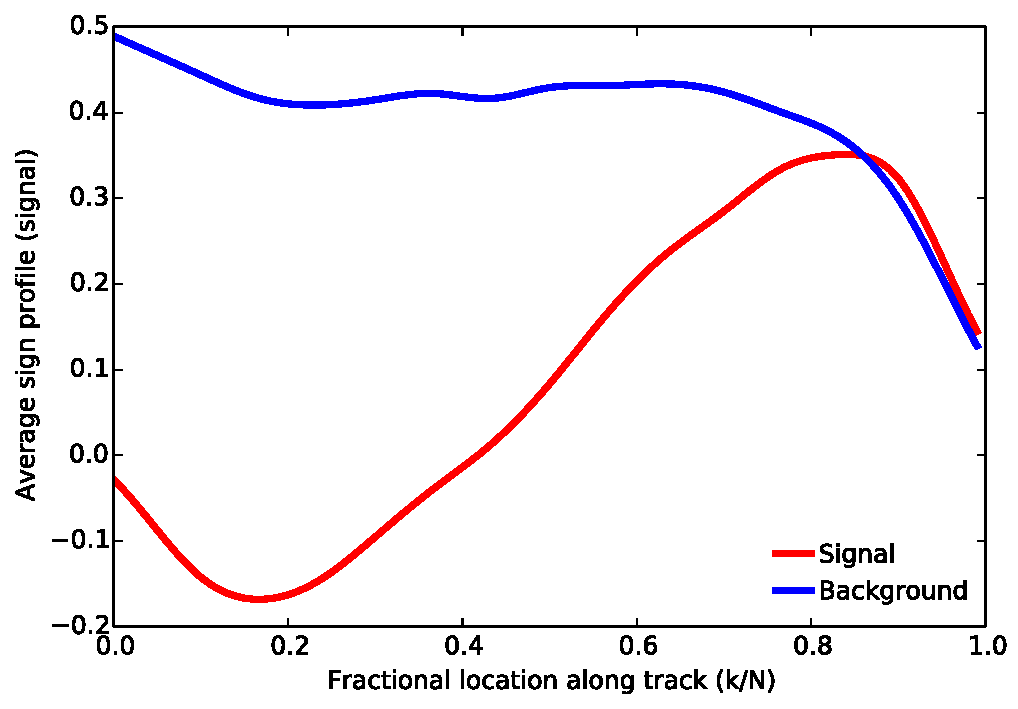
\includegraphics[scale=0.55]{img2/sbprof_nmagse2.pdf}
	\caption{\label{fig_profiles}Average curvature sign profiles for single-electron and $0\nu\beta\beta$ events generated at $B = 0.5$ T and $P = 10$ atm, with $\sigma_{s} = 2$ mm and $N_{s} = 2$.  The profile shows the average sign vs. fractional distance along the track ($k/N$, where $k$ is the hit number and $N$ is the total number of hits).  The profiles were created by dividing the normalized track into 15 bins, and for each calculated curvature value for each event, adding a value of $+1$ or $-1$ to the bin, then dividing each bin by the total number of values placed in it.  The values in the first and second bin were extrapolated linearly to $k/N = 0$, and those in the final two bins were extrapolated to $k/N = 1$.  The entire set of values was then interpolated using cubic polynomials.}
\end{figure}

Once the profiles have been generated, they can be used to define a new variable that will provide separation between the two classes of events.  Figure \ref{fig_svsbprof} compares the signal efficiency obtained for a given background rejection using the profile-based and the method based on the asymmetry factor.  The profile-based method performs better up to a background rejection of about 95\%. Typically a rejection factor of one order of magnitude can be achieved for a signal efficiency of 80\% using the profile method. 

\begin{figure}[!htb]
	\centering
	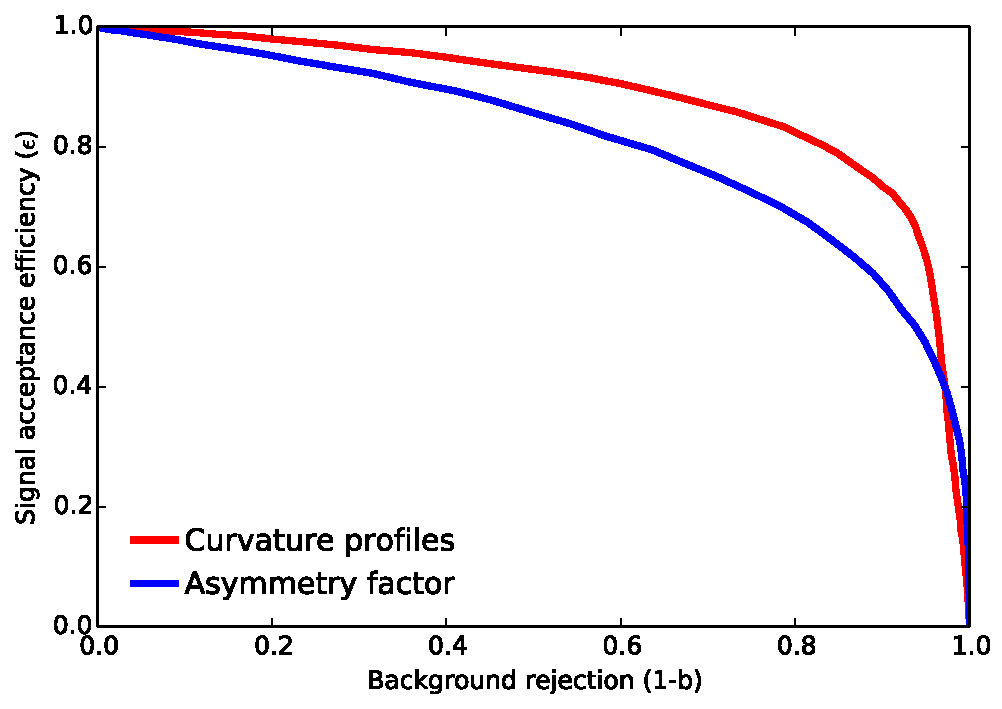
\includegraphics[scale=0.55]{img2/sigvsb_prof_vs_asymm.pdf}
	\caption{\label{fig_svsbprof}Signal acceptance efficiency vs. background rejection obtained at $B = 0.5$ T and $P = 10$ atm, with $\sigma_{s} = 2$ mm and $N_{s} = 2$.  The curve obtained using the curvature asymmetry factor is shown along with that obtained using the profile-based method.}
\end{figure}

The addition of a magnetic field could reduce the background in a ton-scale HPXe well below one count per ton and year, approaching the ``background free'' regime for this scale. On the other hand, the technical difficulties and the costs of adding to the experimental setup a magnet providing a field of around 0.5 Tesla need to be carefully evaluated. 

From the point of view of NEXT R\&D, a test using the NEXT-DEMO detector and the TPC90 magnet, available at CERN (which can run up to 0.7 Tesla) has been approved by the laboratory management. An experimental area has been identified and CERN has agreed to provide the magnet (including water cooling and power) and the infrastructure support. Our schedule foresees to transport NEXT-DEMO and its gas system to CERN in late 2016 and take data in 2017, using several radioactive sources and operating at intensities of 0.1-0.7 Tesla, for about six months.

\subsection{A ton scale HPXe experiment: cost estimate}


\section{The NEXT collaboration}
\label{sec.nc}
 
 \subsection{Organisation of the collaboration}
 
NEXT is an international collaboration including groups from Spain, Portugal, Russia, Colombia and the USA. The project has been headed from its very beginning by a Spanish physicist (J.J. Gomez-Cadenas) and an american physicist (Dave Nygren). The contribution of Dave Nygren (longtime at LBNL, now at University of Texas at Arlington, UTA), Azriel Goldschmidt (LBNL), the late James White (Texas A\&M), Robert Webb (Texas A\&M), and John Hauptman (Iowa State), among others have been essential for the success of the R\&D phase, epitomised by the DEMO and DBDM detectors, the design of the detector, summarised in our TDR \cite{Alvarez:2012sma} and the construction of NEW. Furthermore, NEXT software uses the {\em art} framework, a product developed and maintained by Fermilab, and several Fermilab physicists (notably Adam Para and Paul Lebrun) are currently leading, together with an american Fulbright fellow (Josh Renner) the development of improved reconstruction and pattern recognition algorithms. 

The strong influence of the USA collaboration is recognised explicitly by the nomination of Dave Nygren as International Spokesperson of NEXT and the charge that such role implies. Specifically, while the role of the Spokesperson is to ensure the short-term plans of the collaboration (e.g, the construction, operation and the search for \bbonu\ events of the NEXT-100 detector), the role of the International Spokesperson is to promote the technology as a candidate to explore the IH, as well as seeking to enlarge internationally (and in particular in the USA) the collaboration. 

\subsection{Funding}

NEXT has three sources of funding:
\begin{enumerate}
\item {\bf Funding provided by the Spanish secretary of state for science (SEIDI)}. Spain, as host country of the NEXT-100 experiment, provides the facilities of the Canfranc Underground Laboratory, and has funded the NEXT project during the last seven years, with a total contribution approaching 10 M \euro. 
\item {\bf Funding provided by the European Research Council}, ERC, through an Advanced Grant ($\sim 3$M \euro) awarded to Gomez-Cadenas in 2014.
\item {\bf Funding provided by the international collaboration}. All the NEXT groups contribute to common fund. In addition, the USA contingent has made substantial contributions to the project, both in terms of man power and equipment. 
\end{enumerate}


\subsection{Responsibilities}

The collaboration is currently starting to commission the NEW apparatus. The detector has been fully payed, including a substantial contribution from UTA, which has purchased the SiPMs of the tracking plane and part of the DAQ electronics. The operation and analysis of the detector, as well as the R\&D program (gas mixtures studies with DEMO and NEW, and the operation of DEMO at CERN), require additional contributions from the international collaboration. 

In particular, the USA groups have the following responsibilities in NEW:

\begin{enumerate}
\item F. Monrabal (a UTA postdoctoral associate) is the project leader of the NEW field cage and is in charge of its installation (foreseen for September), commissioning and operation. Monrabal will also be leading the studies with gas mixtures in DEMO.
\item R. Webb (Texas A\&M) has built the electroluminescent amplification system of NEW (EL grid, quartz plate), which is currently being delivered to the LSC. 
\item The Fermilab group is in charge of the general support of the {\em art} framework and lead the development of reconstruction and pattern recognition algorithms (together with Josh Renner).
\item Josh Renner (a LBNL Ph.D., currently a Fulbright Fellow working at IFIC) is leading the studies related with the magnetic field, and will be leading the experimental campaign at CERN.
\end{enumerate}

The NEW effort requires man power from the international collaboration to commission, run and analyse the data.
In particular the contribution of the USA groups is essential for the success of the project. Specifically we propose the following responsibilities for the USA contingent:

\begin{enumerate}
\item {\bf Design engineering}: the design of the NEXT-100 detector was lead by D. Schuman, a senior engineer, then at LBNL. The construction of NEW has followed closely the solutions proposed by the Schuman design, but the construction of NEXT-100, a larger and more complex detector, requires of additional work to review and certify some of the most delicate issues, such as the High Voltage Feedthroughs, the vacuum system of the energy plane, or the design of the field cage (which can be improved to make it more radiopure). 
\item {\bf Energy plane}: The PMTs of NEXT-100 need to operate in vacuum, protected by individual copper enclosures (cans) which are continuously pumped. The construction of such a system requires strong engineering capabilities. We would like the USA groups to take responsibility of the construction and commissioning of the energy plane cans and associated pumping system.  
\item {\bf Field cage}: the field cage is one of the most challenging parts of the detector. Its design was led by Nygren and the late James White, and the construction of the NEW TPC has been lead by F. Monrabal, currently at UTA. We expect that the USA contingent take the full responsibility for the construction, commissioning and operation of the NEXT-100 field cage. 
\item {\bf Software, analysis and data processing}: We would like to strengthen and amplify the current collaboration with Fermilab. In addition to using {\em art} and to the contribution of Fermilab physicists to reconstruction and software, we would like to be able to process Monte Carlo data (huge productions are needed to simulate all the relevant backgrounds) at Fermilab. 
\end{enumerate}

The other key elements of the detector are the pressure vessel, gas system, tracking plane, PMT and SiPM calibration, front-end electronics, DAQ and slow control. Most of these system will be constructed by the Spanish groups, under the leadership of the spokesperson and with help from other international groups. 

Two essential roles in any experiment, in particular during the construction and commissioning phase are that of the Project Manager (PM) and the Technical Coordinator (TC). To reflect the weight of USA in the project, the TC will be taken, starting in 2016, by the UTA group. 
 
\subsection{Time schedule}
\begin{itemize}
\item {\bf 2015:} installation of NEW, start of the R\&D campaign to study gas mixtures with NEXT-DEMO.
\item {\bf 2016:} commissioning and operation of NEW with natural xenon. Studies of energy resolution, electron reconstruction and topological signature. Complete R\&D campaign to study gas mixtures with NEXT-DEMO. Full review of NEXT-100 design. Full test of gas system.
\item {\bf 2017:} Construction of NEXT-100 detector parts: Pressure Vessel and gas system are already in place. The major systems to be built are the energy plane, tracking plane, field cage and inner copper shielding. Installation of NEXT-100 at the LSC.
\item {\bf 2017:} commissioning and operation of NEXT-100 with natural xenon. Full calibration of detector and start of the physics campaign. Operation of NEW with suitable gas mixtures to demonstrate in a large-scale detector the improvement of the topological signature. Test of magnetic field using DEMO at CERN. 
\end{itemize}

\subsection{Man power resources from the USA}

The following list defines a full time scientist (FTS), as a post-doctoral associate, research associate or assistant professor (with no teaching obligations, or the corresponding fraction if teaching obligations are taking into account). FTS do not include typically full professors or senior staff members at universities or national laboratories. A full time engineer (FTE) is defined as a senior engineer who devotes 100\% of his or her time to the project. A Graduate Student (GS) is defined as a USA scientist working for his or her Ph.D. thesis in the NEXT experiment. This list includes resources related with the construction, commissioning and installation (CCI) of the NEW and NEXT-100 detectors, but does not include resourced devoted to the development of software and analysis, where we assume a continuing collaboration with Fermilab. 

\begin{itemize}
\item {\bf 2016:} One FTS, leading the operation of NEW (pure xenon). One FTE working in the NEXT-100 design review. One GS involved in the operation and data analysis of NEW. 
\item {\bf 2017:} Three FTS, one leading the operation of NEW (gas mixtures), one leading the CCI of the NEXT-100 field cage (FC) at UTA, one leading the CCI of the NEXT-100 energy plane (EP) cans and vacuum system (at UTA or elsewhere). One FTE, sharing his or her time between the construction of the FC and the EP. Workshop time and technician man power for the construction of FC and EP.  Two additional GE. One involved in the FC project, the other in the EP project. 
\item {\bf 2018:} Three FTS, involved in the analysis of NEXT-100, the completion of the R\&D (in particular concerning magnetic field) and in the design of a ton-scale HPXe-EL detector.  One FTE, leading the engineering design of the ton-scale detector. One additional GE working in the simulation and design studies of the ton-scale detector as well as in the analysis of NEXT-100 data.
\end{itemize}

\subsection{In-kind contribution from the USA}

\begin{itemize}
\item {\bf Common fund for 2016-2018}: (20 k\$ a year).  
\item {\bf Pays the construction, transport and installation of field cage:} estimated cost 
250 k\$
\item {\bf Pays the construction, transport and installation of energy plane mechanics:} estimated cost 250 k\$.
\item {\bf Contributes to the costs of infrastructures}: 200 k\$.
\item {\bf Contributes to the costs of DAQ and computing}: 150 k\$.
\end{itemize}

In total the contribution of the USA groups for 2016-2018 is estimated in 910 k\$. 
 


 \section{Conclusions}
 \label{sec.conclu}
 In this report we have presented a comprehensive status of the NEXT experiment and its  scientific goals (including R\&D) for the period 2015-2018. Demonstration with the NEW and NEXT-100 detector of the expected performance in energy resolution and background rejection would qualify the technology for a ton-scale detector capable of exploring the IH in a reasonable time (5 year) with a reasonable target mass (2 tons). Furthermore, the collaboration will be pursuing active R\&D to find suitable gas mixtures capable to reduce the diffusion to some 2 mm over 1 m drift length, without jeopardising other capabilities of the detector such as electron lifetime or energy resolution. Promising candidates (Xe + 0.1\% \COT, Xe + 0.5\% \CHF) are currently being investigated. The reduction of diffusion would increase the background rejection of the technique and would open the possibility of further improvement of the topological signature adding a magnetic field. A preliminary estimate of the cost estimate of a ton-scale apparatus yields a figure of 24 M\$ (assuming 15 M\$ for the cost of 1 ton of \XE\ which is a conservative estimate with respect to the cost payed by NEXT). The cost could be increased by perhaps 1 M\$ if a magnet would also be deployed.  
 
 \nocite{*}
\bibliographystyle{elsarticle-num}
\bibliography{biblio}
\end{document}
